\documentclass[11pt]{article}
% -----------------------------------------------------------------------------
% Response to the reviewers of MS CPENG-8674 (major revision, October 2026).
% Draft: answers are written only for the comments addressed so far.
% Code: MODULES/review29oct_fixed | Data: Data/06Nov_FINAL_SlabS10_7D_5sensors_5modes | Figures: ./figures_final
% Orange text = notes for the authors and placeholders (remove or fill before submission).
% -----------------------------------------------------------------------------
\usepackage[a4paper,margin=2.5cm]{geometry}
\usepackage{amsmath,amssymb,bm}
\usepackage{graphicx}
\usepackage{booktabs,multirow,array,longtable,tabularx}
\usepackage{xcolor}
\usepackage{caption,subcaption}
\usepackage{float}
\usepackage{enumitem}
\usepackage{titlesec}
\usepackage{tikz}
\usetikzlibrary{decorations.pathmorphing,arrows.meta,calc,positioning,patterns,decorations.pathreplacing,fit,backgrounds}
\usepackage[round,authoryear]{natbib}
\usepackage[colorlinks=true,linkcolor=blue!50!black,citecolor=blue!50!black,urlcolor=magenta]{hyperref}

\definecolor{resp}{RGB}{25,70,170}
\definecolor{note}{RGB}{205,95,0}
\linespread{1.15}
\setlength{\parindent}{0pt}
\setlength{\parskip}{4pt}
\captionsetup{font=small,labelfont=bf,labelsep=colon}
\renewcommand{\thetable}{R\arabic{table}}
\renewcommand{\thefigure}{R\arabic{figure}}
\renewcommand{\theequation}{R\arabic{equation}}
\titleformat{\section}{\normalfont\large\bfseries}{}{0pt}{}
\titleformat{\subsection}{\normalfont\bfseries}{}{0pt}{}
\setlist{itemsep=1pt,topsep=2pt}

% --- Comment / response / action blocks (as in our previous response letters) ---
\newenvironment{rcomment}[1]{\par\bigskip\noindent\textbf{Comment\ifx&#1&\else\ #1\fi:}\ \itshape}{\par}
\newenvironment{response}{\par\smallskip\noindent\color{resp}\textbf{Response:}\ }{\par}
\newenvironment{action}{\par\smallskip\noindent\color{resp}\textbf{Action:}\ }{\par}
\newcommand{\pending}{\par\smallskip\noindent\textcolor{gray}{\textbf{Response:} \textit{pending --- this comment
has not been addressed yet.}}\par}
\newcommand{\authornote}[1]{\textcolor{note}{\textsf{[Authors: #1]}}}
\newcommand{\tbd}[1]{\textcolor{note}{\textsf{[#1]}}}
\newcommand{\lines}[1]{\tbd{lines #1}}

\newcommand{\m}{\mathbf{m}}
\newcommand{\z}{\mathbf{z}}
\newcommand{\f}{\mathbf{f}}

\begin{document}

\begin{center}
{\Large\bfseries Response to reviewer comments}\\[8pt]
\textbf{MANUSCRIPT ID:} CPENG-8674\\
\textbf{Date:} \today\\
\textbf{Title:} Uncertainty-aware damage identification in short-span bridges via physics-informed variational
autoencoder\\
\textbf{Journal:} Journal of Computing in Civil Engineering
\end{center}

\noindent\fcolorbox{note}{note!6}{\parbox{\dimexpr\linewidth-2\fboxsep-2\fboxrule}{\small\color{note}\textsf{%
\textbf{Draft status (\today).} Answers are given only for the comments addressed so far; the other comments are
reproduced with the mark ``pending''. Orange text is for the authors: notes, and placeholders for the results of the
training on the final dataset and for the line numbers of the revised manuscript. All numbers in blue come from the
final dataset (\texttt{Data/06Nov\_FINAL\_SlabS10\_7D\_5sensors\_5modes}: bridge S10 of Moliner et al., 2017, as a beam on vertical elastic supports; five sensors, five modes) and the scripts in \texttt{MODULES/review29oct\_fixed} and
\texttt{MODULES/baseline\_GaussCopula\_GaussMarginals}.}}}

\bigskip
We would like to thank the three reviewers for the time and effort they devoted to conduct this insightful review.
In the following, we answer each comment point by point. Table~\ref{tab:summary} summarizes the responses and indicates where
the corresponding changes appear in the revised manuscript. Reviewer comments are reproduced in italics, and our responses and the resulting actions are written in blue.

% =============================================================================
\section{Summary of the responses}
% =============================================================================
{\small
\begin{longtable}{p{1.55cm}p{6.0cm}p{3.0cm}p{3.6cm}}
\caption{Point-by-point summary of the responses.}\label{tab:summary}\\
\toprule
Comment & Topic & Status & Revised manuscript \\
\midrule
\endfirsthead
\toprule
Comment & Topic & Status & Revised manuscript \\
\midrule
\endhead
R1.1 & Test data from a finer FE mesh & Addressed & \lines{xx--yy} \\
R1.2 & Model uncertainty and environmental variability & Addressed & \lines{xx--yy} \\
R1.3 & 95\% credible intervals and coverage & Addressed & \lines{xx--yy} \\
R1.4 & Comparison with Refs.\ 39 and 41 & Addressed & \lines{xx--yy} \\
R1.5 & Out-of-distribution test cases & Addressed & \lines{xx--yy} \\
R1.6 & Localized, mild and healthy cases; false positives & Addressed (results pending) & \lines{xx--yy} \\
R1.7 & Finer discretization and scalability & Addressed (results pending) & \lines{xx--yy} \\
R1.8 & Reference list & Addressed & \lines{xx--yy} \\
R2.1 & Utility for real bridges in the introduction & Addressed (draft) & \lines{xx--yy} \\
R2.2 & Realistic structure and elastic bearings & Addressed & \lines{xx--yy} \\
R2.3 & Damage parametrization, support conditions and detectable bearing damage & Addressed (VAE results pending) & \lines{xx--yy} \\
R2.4 & More realistic case study; laboratory beam & Partly addressed (no laboratory data) & \lines{xx--yy} \\
R3.1 & Robustness to modelling error (mass perturbation) & Addressed (results pending) & \lines{xx--yy} \\
R3.2 & Selection of $\gamma$ on the test set & Addressed (sensitivity study pending) & \lines{xx--yy} \\
R3.3 & Prior vs.\ sampling density of the training data & Addressed & \lines{xx--yy} \\
R3.4 & Number of modes and identifiability & Addressed (VAE results pending) & \lines{xx--yy} \\
R3.5 & Flowchart of the data generation and of the offline/online phases & Addressed & \lines{xx--yy} \\
R3.6 & Notation $\mathbf{K}_{\mathrm{G}}$ in Eq.~(11) & Pending & \\
R3.7 & Number of samples $H$ & Addressed & \lines{xx--yy} \\
R3.8 & Hardware and wall-clock time & Pending & \\
\bottomrule
\end{longtable}
}

% =============================================================================
\section{Reviewer \#1}
% =============================================================================
% The authors' notes on which these responses are based are kept in MODULES/_backup_09Nov_letter_user_notes/.

\begin{rcomment}{}
This paper presents a physics-informed Gaussian copula variational autoencoder for uncertainty-aware damage
identification using noisy natural frequencies and mode shapes. Replacing the learned decoder with a differentiable
eigensolver appears to be an interesting approach for end-to-end training, and the manuscript is clearly written. The work
builds on the authors' earlier Gaussian copula VAE (Reference 41) and extends it by embedding the eigensolver and
increasing the latent dimensionality from 2 to 5. The current validation is based on a single five-element synthetic
beam with measurement noise, and I believe that some additional evidence would further strengthen the conclusions
regarding uncertainty quantification, reliability, and scalability. Some clarifications are needed to better understand
the method and its applications.
\end{rcomment}

% -----------------------------------------------------------------------------
\begin{rcomment}{1}
The training and test data are generated using the same five-element model. Could the authors consider testing the trained model on observations generated from a finer mesh while retaining the same five damage zones and sensor locations as in the current paper? This would help assess robustness to model-form uncertainty, since field observations
may not necessarily be well represented by such a coarse discretization.
\end{rcomment}

\begin{response}
We have  built a new, more realistic case study, which also addresses the concerns of Reviewer 2 (R2.2--R2.4). 
The bridge deck is discretized into $n_{e}  = 10$  Euler--Bernoulli beam elements and rests on elastic bearings, represented by vertical springs at both ends (see Fig.~\ref{fig:bridge}). 
The same five damage zones are considered along the deck, and two extra damage features are included for the stiffness of the bearings.  
We employ this 10-element parameterization to generate the training and validation data.
For the test dataset, we employ a finer discretization of the same structure, considering $n_{e} = 50$ elements along the bridge deck (ten elements per zone).
The instrumentation system is kept the same as in the original manuscript. 
%THIS GOES IN R2.
%The latent variables are one stiffness reduction factor per damage zone along the deck, as in the original submission, plus one stiffness factor per bearing (R2.2):
%\begin{equation}
%\hat{\mathbf{K}}_{\mathrm{G}}(\z)=\sum_{d=1}^{5} z_d\sum_{e\in\mathcal{Z}_d}\mathbf{K}_{e}
%+z_{b,L}\,\mathbf{K}_{b,L}+z_{b,R}\,\mathbf{K}_{b,R},
%\label{eq:Kz}
%\end{equation}
%where $\mathcal{Z}_d$ is the set of elements of zone $d$, and $\mathbf{K}_{b,L}$ and $\mathbf{K}_{b,R}$ contain the nominal stiffness of the left (L) and right (R) bearing springs.


%The test damage scenarios are also generated differently from the training ones (R1.5).
%The performance metrics of the identification on the testing dataset are reported in Table~\ref{tab:metricsB} (R1.3).
\end{response}

% -----------------------------------------------------------------------------
\begin{rcomment}{2}
The introduction identifies model uncertainty, measurement error, and environmental variability as sources of
ill-posedness, whereas the numerical study focuses primarily on measurement noise. It would be useful to investigate how
the proposed framework handles the other sources of uncertainty or, alternatively, to discuss this point more explicitly
as a limitation of the present study.
\end{rcomment}

\begin{response}
We have extended the case study to incorporate modeling error.
For that purpose, and responding also to R3.1, we have introduced a mass perturbation in the finite-element parameterization to account for discrepancies with respect to the nominal, reference properties of the system. 
The mass value of each structural element is independently perturbed as: 
\begin{equation}
	m_e^{\text{true}} = m_e^{\text{nom}} \left(1 + \epsilon \xi_e\right), \quad e = 1, \dots, n_{\text{e}},
	\label{eq:modeling_error}
\end{equation}
where $m_e^{\text{nom}}$ denotes the nominal mass value at the $e$-th element, with $n_{e}$ total elements; $\xi_e$ is an independent sample from a standard Gaussian random variable; and $\epsilon$ is the model-error level. 
In this work, we assign a $\epsilon = 0.05$ to represent a $5\%$ error. 
To incorporate this discrepancy, we employ the perturbed values to generate the datasets (observations) while the nominal values are fed as known properties into the physics-informed VAE architecture. 

Besides, the use of a coarse mesh (10-element) for training compared to that used for testing (50-element), as requested by R1.1, introduces an additional source of modeling error (discretization error).

A realistic description of environmental and opeational effects requires long-term monitoring data, which cannot be reproduced reliably in the current synthetic dataset. 
We now specify in the introduction the sources of uncertainty handled in the present work. 
In the conclusions, we describe in more detail the limitations of the methodology, and acknowledge the lack of environmental variability, which is considered as future work as part of the experimental validation. 


%
%We agree that measurement noise is not the only source of uncertainty in practice. The revised study accounts for the
%following sources:
%\begin{enumerate}[leftmargin=*,label=(\alph*)]
%\item \emph{Measurement error.} As in the original submission, the natural frequencies and mode shapes are corrupted
%with Gaussian noise (2.5\% of the frequencies and 5\% of the peak amplitude of the mode shapes).
%\item \emph{Modelling error.} The data are generated with a model that differs from the one used by the SciML method. The
%mass of each 1~m segment of every simulated structure is perturbed as
%\begin{equation}
%\mathbf{M}_e^{\mathrm{data}}=(1+\mu_{s(e)})\,\mathbf{M}_e,\qquad \mu_{s}\sim\mathcal{N}(0,0.05^2),
%\label{eq:asbuilt}
%\end{equation}
%where $s(e)$ is the segment of element $e$, whereas the decoder keeps the nominal mass matrix. Uncertain permanent loads are
%also considered in dynamic studies of short-span bridges (e.g., $\pm30\%$ of the ballast thickness in Moliner et al.,
%2017). In addition, the test data are generated with a finer discretization (50 elements, R1.1) to explore the robustness
%against model-form error.
%\item \emph{Limited information.} We also explore the effect of a scarce measurement data by reducing the number of identified modes (three instead of five), as also requested by Reviewer 3 (R3.4).
%\item \emph{Environmental and operational variability.} A realistic description of these effects requires long-term
%monitoring data, which cannot be reproduced reliably in a synthetic dataset. We acknowledge this as a limitation of the
%present validation and propose an experimental validation that incorporates this source of uncertainty as future work.
%\end{enumerate}

%The statistics of the measurement and modelling errors are estimated by simulation and included in the likelihood (R1.3).
%Note that the objective of the present work is not to disentangle these sources of uncertainty (i.e., to quantify the  contribution of each one), which could be addressed in future work, but to include them to offer a realistic case study
%and a reliable validation.
\end{response}

%\begin{action}
%New paragraph on the sources of uncertainty \lines{xx--yy}, with Eq.~\tbd{x} (Eq.~\eqref{eq:asbuilt}); environmental
%and operational variability discussed as a limitation in the conclusions \lines{xx--yy}.
%\end{action}

% -----------------------------------------------------------------------------
\begin{rcomment}{3}
The abstract reports 77.2\% coverage (line 32), whereas line 352 reports a value of 0.789 for nominal 95\% intervals.
Could the authors clarify how these two values are related? A value below 80\% for nominal 95\% intervals may indicate
some undercoverage. A brief discussion of how the uncertainty intervals are calibrated would therefore be helpful.
\end{rcomment}
\begin{response}
We have entirely updated the results section according to the new case study and corresponding train/validation/test datasets. 
We must also mention that we found an error in the $95\%$ calculation in the submitted version, which produced the undercoverage results. 
In the updated manuscript, we now include (Section ***) the detailed formulation of the performance metrics, and a dedicated table with the obtained results. 
	
For each observation $\m_t$ ($t=1,\dots,N_{\text{test}}$) of the test dataset, with true damage condition
$\z^*_t\in\mathcal{S}=[z_{\text{lb}},z_{\text{ub}}]^{D}$, the encoder provides the parameters of the approximate posterior
$q_{\bm\zeta_{\bm\theta}}(\z|\m_t)$ (Eq.~(8) of the manuscript). The marginal $q_{t,d}$ of each component $d=1,\dots,D$ is
a truncated log-normal distribution: $\ln z_d$ follows a Gaussian distribution with location $\mu_{t,d}$ and scale
$\sigma_{t,d}$, truncated to $[\ln z_{\text{lb}},\ln z_{\text{ub}}]$. Its density and cumulative distribution function
(CDF) are:
\begin{equation}
	q_{t,d}(z)=\frac{\varphi\big((\ln z-\mu_{t,d})/\sigma_{t,d}\big)}{z\,\sigma_{t,d}\,Z_{t,d}},\qquad
	F_{t,d}(z)=\frac{\Psi\big((\ln z-\mu_{t,d})/\sigma_{t,d}\big)-\Psi(\alpha_{t,d})}{Z_{t,d}},\qquad
	z\in[z_{\text{lb}},z_{\text{ub}}],
	\label{eq:marginal_tn}
\end{equation}
where $\varphi$ and $\Psi$ are the standard normal PDF and CDF, $\alpha_{t,d}=(\ln z_{\text{lb}}-\mu_{t,d})/\sigma_{t,d}$,
$\beta_{t,d}=(\ln z_{\text{ub}}-\mu_{t,d})/\sigma_{t,d}$, and $Z_{t,d}=\Psi(\beta_{t,d})-\Psi(\alpha_{t,d})$. Every metric is
averaged over the $N_{\text{test}}\times D$ stiffness factors of the test dataset:
\begin{itemize}[leftmargin=*]
	\item \emph{Mean squared error (MSE) and mean absolute error (MAE)} of the point estimate $\hat z_{t,d}$, the mean of
	the marginal posterior of Eq.~\eqref{eq:marginal_tn}, which has a closed form:
	\begin{equation*}
		\hat z_{t,d}=\int_{z_{\text{lb}}}^{z_{\text{ub}}} z\,q_{t,d}(z)\,\mathrm{d}z
		=e^{\mu_{t,d}+\sigma_{t,d}^2/2}\,\frac{\Psi(\beta_{t,d}-\sigma_{t,d})-\Psi(\alpha_{t,d}-\sigma_{t,d})}{Z_{t,d}},
	\end{equation*}
	\begin{equation}
		\mathrm{MSE}=\frac{1}{N_{\text{test}}D}\sum_{t=1}^{N_{\text{test}}}\sum_{d=1}^{D}\big(\hat z_{t,d}-z^*_{t,d}\big)^2,\qquad
		\mathrm{MAE}=\frac{1}{N_{\text{test}}D}\sum_{t=1}^{N_{\text{test}}}\sum_{d=1}^{D}\big|\hat z_{t,d}-z^*_{t,d}\big|.
		\label{eq:mse_mae}
	\end{equation}
	\item \emph{Average log-likelihood (ALL)} of the true values under the marginal posteriors:
	\begin{equation}
		\mathrm{ALL}=\frac{1}{N_{\text{test}}D}\sum_{t=1}^{N_{\text{test}}}\sum_{d=1}^{D}\log q_{t,d}\big(z^*_{t,d}\big).
		\label{eq:all}
	\end{equation}
	\item \emph{Coverage}: fraction of the true values that lie inside the central credible interval of level $p$, i.e.,
	between the $(1-p)/2$ and $(1+p)/2$ quantiles of the marginal posterior:
	\begin{equation}
		C(p)=\frac{1}{N_{\text{test}}D}\sum_{t=1}^{N_{\text{test}}}\sum_{d=1}^{D}\mathbb{I}\Big[\frac{1-p}{2}\le F_{t,d}\big(z^*_{t,d}\big)\le\frac{1+p}{2}\Big],
		\label{eq:coverage}
	\end{equation}
	where $\mathbb{I}[\cdot]$ equals 1 if the condition holds and 0 otherwise. The 95\% coverage is $C(0.95)$. If the
	posterior is calibrated, $C(p)\approx p$; a lower value (undercoverage) means that the true values fall outside the
	intervals more often than their level indicates.
	\item \emph{Mean absolute calibration error (MACE)} over $n_l=19$ levels $p_l=0.05,0.10,\dots,0.95$:
	\begin{equation}
		\mathrm{MACE}=\frac{1}{n_l}\sum_{l=1}^{n_l}\big|C(p_l)-p_l\big|.
		\label{eq:mace}
	\end{equation}
\end{itemize}
%	The credible intervals are not recalibrated after training: they are the central quantiles of the marginal posteriors
%	predicted by the VAE, and Eqs.~\eqref{eq:coverage} and \eqref{eq:mace} evaluate their calibration.

%	In the submitted version, due to a programming error, the 95\% coverage was computed as
%	\begin{equation*}
%		C_{\text{submitted}}=\frac{1}{N^2D}\sum_{t=1}^{N}\sum_{t'=1}^{N}\sum_{d=1}^{D}
%		\mathbb{I}\big[\mu_{t,d}-1.96\,\sigma_{t,d}\le z^*_{t',d}\le\mu_{t,d}+1.96\,\sigma_{t,d}\big],
%	\end{equation*}
%	i.e., the interval of each test observation $t$ was evaluated at the true values $z^*_{t',d}$ of all the $N$ test
%	observations, instead of only at its own true values ($t'=t$) as in Eq.~\eqref{eq:coverage}. Besides,
%	$\mu_{t,d}\pm1.96\,\sigma_{t,d}$ are the bounds of the 95\% interval of the Gaussian distribution before its
%	truncation to $[z_{\text{lb}},z_{\text{ub}}]$, whereas Eq.~\eqref{eq:coverage} uses the quantiles of the truncated
%	distribution.
Table~\ref{tab:metricsB} reports the metrics on the test dataset. 
%Overall, 87.8\% of the true stiffness factors lie inside their 95\% credible intervals and the MACE is 0.112. 
%The table separates the stiffness factors with intermediate or mild damage ($z^*<0.80$) from the healthy ones and those with light damage ($z^*\ge0.80$). 
%A loss of stiffness below 20\% in
%one zone changes the natural frequencies by about as much as their identification noise or less (R1.6), so the latter are hard to distinguish from each other. The 95\% credible intervals are well calibrated for this second group (coverage	of 0.885) and somewhat too narrow for the damaged factors (0.854), for which the point estimate is also less accurate (MAE of 0.072 against 0.063).
	
	\begin{table}[H]
		\centering\small
		\caption{Performance metrics, Eqs.~\eqref{eq:mse_mae}--\eqref{eq:mace}, on the test dataset (1,200 observations with seven stiffness factors each).}
		\label{tab:metricsB}
		\begin{tabular}{lc}
			\toprule
			Metric & Test dataset \\
			\midrule
			MSE & 0.00716 \\
			MAE & 0.0648 \\
			ALL & 1.558 \\
			95\% coverage, $C(0.95)$ & 0.878 \\
			MACE & 0.112 \\
			\bottomrule
		\end{tabular}
	\end{table}
\end{response}


%

% -----------------------------------------------------------------------------
\begin{rcomment}{4}
References 39 (Gaussian mixture autoencoder) and 41 (Gaussian copula VAE) introduce closely related methods that could
potentially serve as useful baselines. A comparison with these approaches would help assess the benefits of the proposed
strategy more effectively.
\end{rcomment}

\begin{response}
The proposed method builds on two previous works of the authors, Ref.~39 (Gaussian mixture autoencoder) and Ref.~41 (Gaussian copula VAE).
In both works, rather than exactly solved, the forward operator is approximated by an additional neural network (decoder) that acts as a surrogate. 
This approach requires a two-step training strategy, where the approximate forward (surrogate) is first trained independently. 
In the second step, the VAE is trained to find the optimal encoder weights while keeping the decoder weights frozen from the previous step. 
This approach provided good results in our previous works. 
However, it increases the number of trainable parameters and it introduces an extra source of error associated to the forward approximation, whereas in our approach it is solved exactly. 
The accuracy of the surrogate relies on the quantity and quality of the training data, making this approach more sensitive to the design of experiments and data availability.  
In our proposed approach, embedding the exact governing law (eigenvalue problem) to solve the forward endows interpretability to the estimated quantities (stiffness reduction factors) and eliminates the forward error regardless the training data. 
%Another advantage of our approach is the possibility to incorporate new unlabeled measurements (e.g., from an instrumented real structure) into the training process. In the surrogate-based decoder approach, labeled data are needed for the first training step. 

The revised manuscript (Section Results and discussion) includes now a new subsection  to compare the proposed method with the surrogate-based decoder used in  Refs.~39 and~41, including a table with the relevant performance metrics, which can be found also here in Table~\ref{tab:surrogate}.


To conduct this comparison, the eigenvalue solver is replaced by a surrogate neural network, which is pre-trained using the same train/validation datasets. 
The rest of the architecture remains unchanged. 
Table~\ref{tab:surrogate} compares both approaches with the metrics of R1.3, for the training dataset of the case study (14,000 simulations) and for a reduced dataset of 500 simulations drawn at random from it, to analyze the effect of data scarcity in the performance of each approach.
	\begin{table}[H]
		\centering\small
		\caption{Comparison of the surrogate-decoder approach and the proposed method on the
			test dataset.}
		\label{tab:surrogate}
		\footnotesize
		\setlength{\tabcolsep}{4pt}
		\begin{tabular}{llcccccc}
			\toprule
			Simulations & Decoder & \shortstack{Learnable\\parameters} & MSE & MAE & ALL & $C(0.95)$ & MACE \\
			\midrule
			14,000 & Surrogate-based decoder          & 88,946 & 0.00716 & 0.0646 & 1.564 & 0.880 & 0.109 \\
			       & Eigenvalue solver (proposed) & 75,306 & 0.00716 & 0.0648 & 1.558 & 0.878 & 0.112 \\
			       & $\Delta$                     &        & $+0.0\%$ & $+0.2\%$ & $-0.4\%$ & $-0.2\%$ & $+2.2\%$ \\
			\midrule
			500    & Surrogate-based decoder          & 88,946 & 0.00883 & 0.0737 & 1.335 & 0.836 & 0.168 \\
			       & Eigenvalue solver (proposed) & 75,306 & 0.00826 & 0.0694 & 1.466 & 0.860 & 0.132 \\
			       & $\Delta$                     &        & $\mathbf{-6.4\%}$ & $\mathbf{-5.8\%}$ & $\mathbf{+9.9\%}$ & $\mathbf{+2.9\%}$ & $\mathbf{-21.5\%}$ \\
			\bottomrule
		\end{tabular}
	\end{table}
	
	%This, and maybe also the table, could be ommitted here and appear only in the paper. However, i think it may be useful to find them here. 
In the Table, the value $\Delta$ indicates the relative change of each metric when the surrogate of Ref.~41 is replaced by the proposed eigenvalue solver.
With 14,000 simulations, both approaches give comparable metrics, i.e., the surrogate is accurate enough when it is trained with a large dataset covering the entire parameter space. However, with 500 simulations, the proposed method outperforms the surrogate approach in every metric (Table~\ref{tab:surrogate}): it reduces the error metrics (MSE by 6.4\%, MAE by 5.8\% and MACE by 21.5\%) and yields a higher ALL (+9.9\%) and  95\% coverage (from 0.836 to 0.860).
	While the MSE and MAE only evaluate the error of the point estimate, i.e., the posterior mean, the MACE evaluates the calibration of the whole posterior: it averages, over $n_{l}$ credibility levels, the absolute difference between the nominal level and the fraction of true values that lie inside the corresponding credible intervals (Eq.~\eqref{eq:mace}), so it vanishes when the uncertainty stated by the posterior matches the actual errors.
	With 500 simulations, the credible intervals of both approaches have the same mean width, but those of the surrogate approach contain the true values less often at every level. 
	The approximation error of the surrogate displaces its posterior, but this error is not represented in the likelihood, so the posterior does not widen to account for it and becomes overconfident. 
	Hence, replacing the surrogate by the exact eigenvalue solver improves mainly the reliability of the uncertainty quantification, which is the main purpose of the method, and only moderately the point estimate, mainly for scarce training datasets.


%The outperformance is expected to increase when the effect of damage on the measurements is small compared with the effect of noise, as for early-stage damage (R1.6), since a small error of the surrogate may mask the effect of the damage.

%We expect this advantage to be larger in more complex problems, in which the forward operator is harder to approximate with a given number of simulations: more latent variables (damage zones), more measured outputs (modes and sensors), or more detailed FE models whose cost limits the number of simulations available to train the surrogate.
%The advantage is also expected to increase when the effect of damage on the measurements is small compared with the noise, as for early-stage damage (R1.6), since then even a small error of the surrogate is comparable to the effect of the damage itself.


Besides, in Ref.~39, the posterior is approximated with a Gaussian mixture. This approach has been extensively compared to Gaussian copulas in the recent Ref.~41, where the copula reached an accuracy comparable to that of Gaussian mixtures with full covariance matrices at a lower computational cost.	This advantage grows with the dimension $D$ of the latent space: a mixture of $G$ Gaussians with full covariance matrices requires $G\,(1+D+D(D+1)/2)-1$ parameters to describe the posterior, against $2D+D(D-1)/2$ for the Gaussian copula (179 against 35 for $G=5$ and the $D=7$ latent variables of the present case study, see also R1.7).
For these reasons, the authors consider the comparison against Gaussian mixtures sufficiently analyzed in Ref.~41 to support the use of copulas, and do not repeat it here.


	% ---- previous longer version (KL divergence, advantages, physics figure), kept for reference ----
%	For a quantitative comparison, we have implemented the approach of Ref.~41 for the present problem: the eigenvalue solver is replaced by a surrogate NN with the architecture of Ref.~41, pre-trained with the FE responses at the damage states of the training dataset and then frozen. The rest of the method is unchanged.
%	Besides the performance metrics of R1.3, which measure the distance to the true stiffness factors, we measure how far the approximate posterior $q(\z\mid\m_t)$ of each approach is from the exact Bayesian posterior $p(\z\mid\m_t)$, with the Kullback--Leibler divergence estimated by importance sampling with the exact FE model:
%	\begin{equation}
%		D_t=\log\Big(\frac{1}{S}\sum_{s=1}^{S}w_s\Big)-\frac{1}{S}\sum_{s=1}^{S}\log w_s,\qquad
%		w_s=\frac{p(\m_t\mid\z_s)\,p(\z_s)}{q(\z_s\mid\m_t)},\quad \z_s\sim q(\z\mid\m_t),
%		\label{eq:kl_exact}
%	\end{equation}
%	with $S=500$ samples per test observation. $D_t$ is a lower bound of $\mathrm{KL}\big(q(\z\mid\m_t)\,\|\,p(\z\mid\m_t)\big)$, it is zero when the approximate posterior coincides with the exact one, and it is computed in the same way for both approaches. Table~\ref{tab:surrogate} reports its mean $\bar D$ over the test dataset, together with the metrics of R1.3, the false-alarm rate of R1.6 and the number of learnable parameters, for the training dataset of the case study (14,000 simulations) and for a reduced training dataset of 500 simulations drawn at random from it.

%	\begin{table}[H]
%		\centering\small
%		\caption{Comparison of the proposed method (eigenvalue solver) with the approach of Ref.~41 (surrogate decoder) on the
%			test dataset, with the same posterior model, encoder, likelihood and convergence rule, for two sizes of the
%			training dataset. Metrics as defined in R1.3; false-alarm rate as defined in R1.6; $\bar D$: mean divergence
%			from the exact posterior, Eq.~\eqref{eq:kl_exact} (0 for the exact posterior).}
%		\label{tab:surrogate}
%		\footnotesize
%		\setlength{\tabcolsep}{3pt}
%		\begin{tabular}{llcccccccc}
%			\toprule
%			\shortstack{Simu-\\lations} & Decoder & \shortstack{Learnable\\parameters} & MSE & MAE & ALL & MACE & $C(0.95)$ & \shortstack{False\\alarms} & $\bar D$ \\
%			\midrule
%			14,000 & Eigenvalue solver & 75,306 & 0.00716 & 0.0648 & 1.558 & 0.112 & 0.878 & 2.6\% & 0.068 \\
%				   & Surrogate         & 88,946 & 0.00716 & 0.0646 & 1.564 & 0.109 & 0.880 & 2.6\% & 0.077 \\
%			\midrule
%			500    & Eigenvalue solver & 75,306 & 0.00826 & 0.0694 & 1.466 & 0.132 & 0.860 & 3.3\% & 0.968 \\
%				   & Surrogate         & 88,946 & 0.00883 & 0.0737 & 1.335 & 0.168 & 0.836 & 4.4\% & 1.156 \\
%			\bottomrule
%		\end{tabular}
%	\end{table}

%	With 14,000 simulations, the surrogate reproduces the natural frequencies of the eigenvalue solver within 0.2\% on average (Table~\ref{tab:forward}), well below the measurement noise, and both approaches identify the damage with practically the same metrics. Nevertheless, the posterior of the proposed method is closer to the exact one ($\bar D$ of 0.068 against 0.077), since the residual error of the surrogate enters the likelihood.

%	With 500 simulations, the surrogate approximates the forward operator worse (Table~\ref{tab:forward}), and this additional error degrades every metric of the surrogate approach, including the divergence from the exact posterior (1.156 against 0.968). The proposed method is affected by the smaller dataset only through its encoder, since its forward operator remains exact. The degradation of the surrogate approach is largest for the healthy and lightly damaged stiffness factors, whose effect on the frequencies is of the order of the measurement noise (R1.6): there, an error of the forward operator is comparable to the effect of the damage itself.

%	Beyond these results, embedding the eigenvalue solver provides the advantages of a known, fixed forward operator stated in the introduction of the manuscript:
%	\begin{itemize}[leftmargin=*]
%		\item \emph{Physical meaning of the latent variables.} The decoder is the FE model itself: the latent variables scale the stiffness matrices of the damage zones and bearings (Eq.~\eqref{eq:Kz}), so the identified variables are exactly the stiffness factors that explain the measurements, and their sensitivities $\partial f/\partial z_d$, which drive the training of the encoder, are exact. With a surrogate, they are the inputs of a black-box approximation, whose sensitivities differ from those of the FE model even where its frequencies are accurate.
%		\item \emph{Physically consistent predictions.} The eigenvalue solver satisfies the physical laws of the FE model by construction, whereas the surrogate only approximates them (Fig.~\ref{fig:physics}): it may predict a lower natural frequency for a stiffer zone, which violates Rayleigh's principle, and different frequencies for two mirror-image damage scenarios of the symmetric bridge.
%		\item \emph{Validity for any damage state.} The eigenvalue solver is exact for any damage state, whereas the surrogate is only accurate inside the domain and with the amount of its training data (Table~\ref{tab:forward}).
%		\item \emph{No surrogate to train.} The proposed method is trained in a single step with the measured modal data only: it requires neither a labelled dataset of damage states and FE responses, nor selecting and training a surrogate, nor retraining it when the FE model, the sensors or the selected modes change, and it has fewer learnable parameters (Table~\ref{tab:surrogate}).
%	\end{itemize}
%	\begin{table}[H]
%		\centering\small
%		\caption{Difference between the natural frequencies computed by the surrogate decoder (architecture of Ref.~41) and
%			by the eigenvalue solver of the proposed method, which is exact for the FE model: mean, 95th percentile and maximum
%			over all modes and damage states, and share of damage states in which the difference of at least one frequency
%			exceeds the measurement noise (2.5\%). The training domain is $[0.45,1]^7$.}
%		\label{tab:forward}
%		\footnotesize
%		\begin{tabular}{llcccc}
%			\toprule
%			Damage states & Simulations & Mean & 95th perc. & Max. & Above noise \\
%			\midrule
%			Inside the training domain & 14,000 & 0.19\% & 0.50\% & 4.3\% & 0.1\% \\
%			 & 5,000 & 0.28\% & 0.75\% & 5.2\% & 0.4\% \\
%			 & 2,000 & 0.57\% & 1.60\% & 6.9\% & 3.5\% \\
%			 & 1,000 & 0.76\% & 2.21\% & 7.8\% & 9.1\% \\
%			 & 500 & 0.99\% & 2.94\% & 15.1\% & 17.7\% \\
%			\midrule
%			One deck zone with $z_d\in[0.20,0.45)$ & 14,000 & 1.45\% & 5.45\% & 18.3\% & 49.9\% \\
%			Bearings with $z_b\in(1,3]$ & 14,000 & 4.63\% & 12.47\% & 31.2\% & 93.4\% \\
%			\bottomrule
%		\end{tabular}
%	\end{table}
%	\begin{figure}[H]
%		\centering
%		\includegraphics[width=\textwidth]{figures_final/Fig_surrogate_physics.pdf}
%		\caption{Physical laws that the eigenvalue solver satisfies by construction and the surrogate decoder does not (20,000 damage states drawn uniformly over the training domain). (a) Frequency of mode 2 vs the stiffness factor of zone 1, with the other factors fixed at $(z_2,\dots,z_5,z_{b,L},z_{b,R})=(0.45,0.65,0.48,0.80,0.48,0.49)$: the case with the most decreasing steps of the surrogate among 2,100 random sweeps. (b) Share of cases in which a 5\% stiffer zone or bearing gets a lower natural frequency, which is impossible (Rayleigh's principle). (c) Mean difference between the frequencies of mirror-image damage scenarios, which are identical in the symmetric bridge.}
%		\label{fig:physics}
%	\end{figure}
%		Once trained, both approaches identify the damage with the encoder only, at the same cost.

%	The revised manuscript (Section Results and discussion) includes a new table that compares both approaches with the performance metrics of R1.3 (MSE, MAE, ALL, MACE and 95\% coverage) for the two training datasets, as in Table~\ref{tab:surrogate}.


	
	
	%	
	%The proposed method builds on two previous works of the authors, Ref.~39 (Gaussian mixture autoencoder) and Ref.~41
	%(Gaussian copula VAE), and differs from them in two components (Table~\ref{tab:refs}):
	%\begin{enumerate}[leftmargin=*,label=(\roman*)]
	%\item \emph{Decoder.} Refs.~39 and 41 approximate the forward operator with a neural network (surrogate model) that is
	%pre-trained on simulated data and then frozen while the encoder is trained. The proposed method embeds a differentiable
	%eigenvalue solver that computes the forward problem exactly, without trainable parameters and without a pre-training
	%step.
	%\item \emph{Posterior model.} Ref.~39 describes the posterior with a Gaussian mixture, whereas Ref.~41 and the proposed
	%method use a Gaussian copula.
	%\end{enumerate}
	%
	%\textit{Comparison with Ref.~41 (decoder).} Since Ref.~41 and the proposed method share the posterior model, a comparison
	%with Ref.~41 isolates the effect of the decoder. We implemented the approach of Ref.~41 for the present problem: the
	%eigenvalue solver is replaced by a fully connected surrogate with the architecture of Ref.~41, which is first trained, at
	%the damage states of the same training dataset, to reproduce the natural frequencies and mode shapes computed with the FE
	%model. Its weights are then frozen,
	%and the encoder is trained exactly as in the proposed method (same dataset, encoder, posterior model, likelihood and
	%training protocol). The surrogate introduces an additional approximation error in the forward model, which the likelihood
	%does not account for, and requires a second training step and additional parameters. We compare both approaches in terms of
	%the accuracy of the decoder, the agreement of the approximate posterior with the exact posterior, the metrics of the
	%manuscript on both test sets, and the computational cost (Table~\ref{tab:surrogate}).
	%
	%
	%\textit{Comparison with Ref.~39 (posterior model).} Gaussian mixtures and the Gaussian copula were already compared in
	%Ref.~41: the copula reached an accuracy comparable to that of Gaussian mixtures with full covariance matrices at a lower
	%computational cost, mixtures with diagonal covariance matrices were less accurate because they cannot capture the
	%correlations between the latent variables, and increasing the number of mixture components did not improve the results.
	%The differences grow with the dimension $D$ of the latent space. For the seven latent variables of the revised case study, a
	%mixture of $G=5$ Gaussians with full covariance matrices requires $G\,(1+D+D(D+1)/2)-1=179$ parameters per observation,
	%against $2D+D(D-1)/2=35$ for the Gaussian copula, and its truncation to the support of the prior involves the joint
	%seven-dimensional distribution instead of seven one-dimensional marginals. For these reasons, we do not repeat this
	%comparison here, and the revised manuscript summarizes the findings of Ref.~41.
	
	
\end{response}


% -----------------------------------------------------------------------------
\begin{rcomment}{5}
All test cases appear to be sampled from the same distribution as the training data. It would be helpful to include several additional cases where the test data fall outside the training distribution to illustrate how the proposed method behaves under distribution shift.
\end{rcomment}

\begin{response}
According to the requirements of Reviewer 2, we now employ a more realistic finite element  parametrization that includes vertical bearings at both ends of the bridge. 
The damage condition is described by the stiffness factors of two types of structural components: $n_z$ damage zones
along the deck, each comprising one or several consecutive elements, and $n_b$ bearings, represented by vertical springs.
The global stiffness matrix is assembled in the standard way from the element matrices, each one scaled by the
stiffness factor of its component:
\begin{equation}
	\hat{\mathbf{K}}_{\mathrm{G}}(\z)=\sum_{k=1}^{n_z} z_k\sum_{e\in\mathcal{Z}_k}\mathbf{L}_e^{\top}\mathbf{K}_e\,\mathbf{L}_e
	+\sum_{r=1}^{n_b} z_{n_z+r}\,k_r\,\bm{\ell}_r\bm{\ell}_r^{\top},
	\label{eq:Kz}
\end{equation}
where $\mathbf{K}_e$ is the stiffness matrix of element $e$ in its local degrees of freedom (DOFs), $\mathbf{L}_e$ is the
Boolean connectivity matrix that extracts the DOFs of element $e$ from the global DOF vector, $\mathcal{Z}_k$ is the set of
elements of the $k$-th deck zone, $k_r$ is the nominal stiffness of the vertical spring of the $r$-th bearing, and
$\bm{\ell}_r$ is the unit vector that selects the vertical DOF of its support node. Hence, $\mathbf{L}_e^{\top}\mathbf{K}_e
\mathbf{L}_e$ is the element matrix expanded to the global dimensions, with zeros at the DOFs that do not belong to the
element, and $z_k$ and $z_{n_z+r}$ are the
stiffness factors of the $k$-th deck zone and of the $r$-th bearing. The damage condition vector
$\z=\{z_1,\dots,z_D\}^{\top}$ therefore gathers the $D=n_z+n_b$ stiffness factors, and Eq.~\eqref{eq:Kz} can be written
compactly as $\hat{\mathbf{K}}_{\mathrm{G}}(\z)=\sum_{d=1}^{D}z_d\,\mathbf{K}_d$, where $\mathbf{K}_d$ is the nominal
contribution of the $d$-th component to the global stiffness matrix. In the case study, $n_z=5$ deck zones and $n_b=2$
bearings (left and right, with stiffness factors $z_{b,L}\equiv z_6$ and $z_{b,R}\equiv z_7$), so $D=7$.

To generate the damage scenarios, we have modified the design of experiments according to R1.6 and R2.3 to generate localized damage scenarios and to account also for the bearings. 
In addition to using a different discretization level (See R1.1), the design of experiments has been conducted differently for (a) the training/validation data and (b) the test data. 

\begin{itemize}[leftmargin=*]
	\item \emph{Train/validation data (10-element model):} The same reduction factor $z_d$ multiplies all the bending stiffness of the elements in zone $d$ (Eq.~\eqref{eq:Kz}), so the damage is spread uniformly over the entire zone. 
	
	\item \emph{Test dataset:} Each test scenario is defined by the reduction factors $z_d \in \mathbf{z}$, but in every damaged zone ($z_d<0.95$) the loss of stiffness is concentrated in a damaged region of length $\ell_d$, at a random position within the zone, while the rest of the zone keeps its nominal stiffness.
	The stiffness factor $s$ of the damaged region is chosen so that the zone keeps the same overall stiffness as a zone
	uniformly damaged with factor $z_d$, as in the training data. Under bending, the segments of a zone behave like springs
	in series: their flexibilities, proportional to $(L/EI)_{d}$, add up. If a fraction $\alpha=\ell_d/L_{d}$ of the zone has
	stiffness factor $s$ and the rest keeps its nominal stiffness, both zones are equally flexible when
	\begin{equation}
		\frac{1}{z_d}=\frac{\alpha}{s}+(1-\alpha)
		\qquad\Longrightarrow\qquad
		s=\frac{\alpha\,z_d}{1-(1-\alpha)\,z_d}.
		\label{eq:localized}
	\end{equation}
	This is the usual way of representing a crack or a localized loss of stiffness in a beam as a short segment with reduced $EI_d$ \citep[e.g.,][]{sinha2002simplified}. For 	$\alpha=1$, the damage is uniform and $s=z_d$, whereas a shorter damaged region requires a larger local loss of stiffness; e.g., a zone with $z_d=0.6$ can be damaged over 0.4~m with $s=0.23$, or over 1.0~m with $s=0.43$.
	In the 50-element test model, the damaged region consists of $n$ contiguous elements of 0.2~m ($\alpha=n/10$), with a random position within the zone, and $n$ is drawn among the values that keep $s\ge0.15$ (at most 85\% of local stiffness loss), so that severe damage is not concentrated in an unrealistically short region.
	Undamaged deck zones and bearings are imposed as in the training data.
\end{itemize}
This approach allows us to create different damage scenarios that are realistic (e.g., effect of cracking) while preserving a controlled and representative design of experiments for the train/validation datasets. 
All the test results included in the revised manuscript correspond to this dataset. 
%All the test results in the revised manuscript (e.g., Tables~\ref{tab:metricsB} and~\ref{tab:surrogate}), including the benchmark scenarios whose posteriors are plotted, are obtained with these out-of-distribution test scenarios.
\end{response}



 
%In both cases, the damage condition is described by the stiffness factors of $D$ structural components: $n_z$ damage zones along the deck, each comprising one or several consecutive elements, and the two bearings ($D=n_z+2$). The updated global stiffness matrix is
%\begin{equation}
%\hat{\mathbf{K}}_{\mathrm{G}}(\z)=\sum_{d=1}^{n_z} z_d\sum_{e\in\mathcal{Z}_d}\mathbf{K}_{e,\mathrm{G}}
%+z_{b,L}\,\mathbf{K}_{b,L}+z_{b,R}\,\mathbf{K}_{b,R}=\sum_{d=1}^{D}z_d\,\mathbf{K}_d,
%\label{eq:Kz}
%\end{equation}
%where $\mathcal{Z}_d$ is the set of elements of zone $d$, $\mathbf{K}_{b,L}$ and $\mathbf{K}_{b,R}$ contain the nominal
%stiffness of the left and right bearing springs, and $\mathbf{K}_d$ is the nominal stiffness matrix of the $d$-th
%component expanded to the global dimensions (with $z_{n_z+1}\equiv z_{b,L}$ and $z_{n_z+2}\equiv z_{b,R}$). In the case
%study, $n_z=5$ and $D=7$. 
%Besides the finer discretization of the test data (50 elements instead of 10, R1.1), we create the damage scenarios differently with an equivalent stiffness reduction:

% -----------------------------------------------------------------------------
\begin{rcomment}{6}
The paper introduces damage by sampling from a uniform distribution (line 323), which appears to result in substantial
stiffness reduction in most or all five elements simultaneously. Since structural damage is often localized, it would be
valuable to also evaluate healthy cases and cases with mild damage affecting only one or two elements. Reporting the
corresponding false-positive behavior would further support the manuscript's emphasis on early damage identification.
\end{rcomment}

\begin{response}
We have defined a new design of experiments to create the damage scenarios, including not only distributed damage, but also localized cases (affecting one or two zones only). 
%The strategy described in R1.5 to create localized test scenarios of equivalent stiffness within a certain zone also contributes to this concern. 

To generate the datasets, we have classified the scenarios by the number of damaged components or zones. 
Each zone (here a deck region or a bearing) has one stiffness factor $z_d$, and it is considered damaged when its stiffness factor is below the health limit $\eta=0.95$, i.e., $z_d<\eta$. 
The total generated $N$ samples are divided into categories $c$, defined by the number of damaged components, with $N_c=\pi_c N$ samples each (see Table~\ref{tab:doe}), and each sample $i$ of a category is assigned a set $\mathcal{A}^{(i)}$ of damaged components. 
All the possible sets with the number of damaged components of the category are assigned cyclically, in random order, so that every component and every combination of components is damaged the same number of times. 
The stiffness factors are then
\begin{equation}
z_d^{(i)}=
\begin{cases}
z_{lb}+(\eta-z_{lb})\,\dfrac{p_d^{(i)}+u_d^{(i)}}{N_{c,d}}, & d\in\mathcal{A}^{(i)},\\[2ex]
\eta+(1-\eta)\,u_d^{(i)}, & d\notin\mathcal{A}^{(i)},
\end{cases}
\qquad u_d^{(i)}\sim\mathcal{U}(0,1),
\label{eq:doe}
\end{equation}
where $N_{c,d}$ is the number of samples of category $c$ in which component $d$ is damaged and $p_d^{(i)}$ is a random
permutation of $\{0,\dots,N_{c,d}-1\}$ over these samples. The severities of the damaged components are thus stratified
(Latin hypercube) over $[z_{lb},\eta)$, from the most severe damage considered to very slight damage, and the
undamaged components lie in $[\eta,1]$, which represents the healthy state with small as-built variations.

The dataset focuses on localized damage, which is the most realistic situation and the case requested by the reviewer:
\begin{itemize}[leftmargin=*]
\item \emph{Few damaged components.} Most of the scenarios have only one (30\%) or two (25\%) damaged components, and 10\%
are healthy structures (Table~\ref{tab:doe}). Scenarios with three to five damaged components and a category drawn
uniformly over the whole parameter space complete the dataset, so that the method is also trained on distributed damage.
The validation and test datasets follow the same proportions: the test dataset contains 120 healthy structures and 661
structures with one or two damaged components.
\item \emph{Light and very slight damage.} The severities are spread uniformly down to very slight damage: 30\% of the
damaged components have a loss of stiffness below 20\% ($0.80\le z_d^*<0.95$).
\item \emph{Damage localized within the component.} In the test dataset, the loss of stiffness of a damaged zone is
concentrated in a region of one to ten contiguous elements of 0.2~m (0.2 to 2~m) at a random position, while the rest of
the zone keeps its nominal stiffness (R1.5). The test scenarios therefore include damage affecting only one or two
elements of the FE model, as suggested by the reviewer.
\end{itemize}
The lower bound $z_{lb}=0.45$ corresponds to a maximum loss of stiffness of 55\%, so extremely severe damage is not
considered in this work: the study focuses on damage of intermediate to very slight severity, which is the relevant
range for early damage identification.

\begin{table}[H]
\centering\small
\caption{Categories of the design of experiments (Eq.~\eqref{eq:doe}). Components: five deck zones and two bearings.}
\label{tab:doe}
\begin{tabular}{lcc}
\toprule
Category & Share $\pi_c$ & Number of damaged components \\
\midrule
Healthy & 10\% & 0 \\
Single damage & 30\% & 1 \\
Double damage & 25\% & 2 \\
Triple damage & 15\% & 3 \\
Multiple damage & 10\% & 4 or 5 \\
Uniform & 10\% & $\z\sim\mathcal{U}[z_{lb},1]^D$ \\
\bottomrule
\end{tabular}
\end{table}

\textit{From the posterior to a decision.} The method estimates the location and severity of damage with a posterior
distribution of every stiffness factor, whereas false positives and false negatives refer to a binary decision (damaged
or healthy) for each component. We obtain this decision from the point prediction used for the MSE and MAE of R1.3, the
posterior mean $\hat z_d$: component $d$ is declared damaged when $\hat z_d<\tau$. A false positive is a healthy component
($z_d^*\ge\eta$) declared damaged, and a false negative is a component with a loss of stiffness larger than 20\%
($z_d^*<0.80$) declared healthy. Components with light damage ($0.80\le z_d^*<\eta$), whose effect on the measurements is
of the order of the noise (see below), are not counted in either rate. The threshold $\tau$ must therefore lie between
0.80 and $\eta$, and its value sets the balance between both errors: a higher threshold declares more components damaged,
which reduces the false negatives but increases the false positives, and vice versa. Since both errors are considered
equally undesirable, we select the threshold that makes both rates equal on the validation dataset (equal-error-rate
criterion, a standard choice in detection problems), $\tau=0.84$, and then apply it unchanged to the test dataset. The ROC
curve of Fig.~\ref{fig:roc} shows the rates obtained with any other threshold.

\textit{Results.} On the test dataset, the false-positive rate is 8.3\% and the false-negative rate is 9.9\%. In the
120 healthy structures, 4.3\% of the components are false positives. Fig.~\ref{fig:roc} shows the ROC curve obtained by
varying $\tau$, with an area under the curve (AUC) of 0.97.

\begin{figure}[H]
\centering
\includegraphics[width=0.5\textwidth]{figures_final/Fig_ROC_components.pdf}
\caption{ROC curve of the classification of the components of the test structures (healthy, $z_d^*\ge0.95$, against
damaged, $z_d^*<0.80$) with the posterior mean $\hat z_d<\tau$; the marker shows the threshold $\tau=0.84$ selected on
the validation dataset.}
\label{fig:roc}
\end{figure}

\textit{Origin of the errors: noise and sensitivity.} Distinguishing a healthy component from a lightly damaged one is
limited by two physical factors. First, the measurement noise: a loss of stiffness below 20\% in one component changes
the natural frequencies by about as much as, or less than, their identification noise and the modelling errors (mass
distribution, finer discretization and localized damage), so the measurements of a lightly damaged structure are also
compatible with a healthy one, and vice versa. Second, the sensitivity of the measurements, which depends on the
location of the component: the two deck end zones concentrate most of the false positives and half of the false
negatives. Near the supports the bending moment is small in every mode, so little strain energy is
stored in the end zones and the natural frequencies are several times less sensitive to their stiffness than to that
of the interior zones; in addition, a loss of stiffness of an end zone and a softer bearing have a similar effect on the
modal data. When the measurements are
insensitive to a component, its posterior remains wide and close to the uniform prior, so its posterior mean is pulled
towards the prior mean (0.725), which explains the false positives in healthy end zones. The false negatives are mostly
mild damage, with a loss of stiffness between 20\% and 30\%, whose posterior mean lies just above the threshold. We
consider the false-positive and false-negative rates admissible: both are below 10\% and balanced, the errors
concentrate on the mildest relevant damage and on the least sensitive locations, and, in a monitoring context, the
identification is repeated over time, so that a damage that grows is detected in subsequent tests.

\textit{Representative cases.} To illustrate these results, we selected representative cases of the test dataset.
Fig.~\ref{fig:cases_well} shows four cases that are well identified: (a) a healthy bridge, with every component declared
healthy and posteriors concentrated near the healthy state; (b) light damage in an interior zone, whose posterior mean
coincides with the true value, although its credible interval still includes healthy values, as expected for light
damage; (c) damage in one bearing and (d) damage in two adjacent interior zones, which are correctly located and
quantified, without false positives. Fig.~\ref{fig:cases_fail} shows the typical failures, which involve the deck end
zones: (a) a healthy bridge with a false positive in end zone 1; (b) a severe damage concentrated next to the right
support that is not detected, since the bending moment of every mode vanishes at the support, whereas (d) the same
equivalent damage distributed over the whole zone (10-element test data, in which the damage is uniform within each
zone) is detected and correctly quantified; and (c) a damage in end
zone 1 that is partly attributed to the left bearing, which produces a false negative in the zone and a false positive
in the bearing.

\begin{figure}[H]
\centering
\includegraphics[width=\textwidth]{figures_final/Fig_cases_well.pdf}
\caption{Posteriors of the stiffness factors (violin plots) of four well-identified cases of the test dataset, with
the decision of each component ($\hat z_d<0.84$: declared damaged).}
\label{fig:cases_well}
\end{figure}

\begin{figure}[H]
\centering
\includegraphics[width=\textwidth]{figures_final/Fig_cases_fail.pdf}
\caption{Posteriors of the stiffness factors (violin plots) of three cases of the test dataset with wrong decisions
(a--c), and of the structure of case (b) with the same equivalent damage uniformly distributed over zone 5 (d), with
the decision of each component ($\hat z_d<0.84$: declared damaged).}
\label{fig:cases_fail}
\end{figure}

\textit{Added value of the posterior distribution.} False-positive and false-negative rates only assess the point
prediction. The posterior distribution also quantifies how reliable each decision is: the wrong decisions correspond to
wide posteriors, and the 95\% credible intervals of the healthy components declared damaged are, on average, almost
twice as wide as those of the healthy components declared healthy. In Fig.~\ref{fig:cases_fail}(a), the false positive
has a wide posterior that contains the true, healthy value, and in Fig.~\ref{fig:cases_fail}(c) the true stiffness
factor of the undetected damage also lies inside the wide posterior of end zone 1. A deterministic estimate would give
the same wrong decisions without any indication of their reliability, whereas the posterior shows that these decisions
are uncertain and should be confirmed (e.g., by inspection or further measurements) before acting.

The limit imposed by noise on single tests is well known in vibration-based monitoring: the smallest detectable
damage is bounded by the identification uncertainty of the modal parameters, and the literature lowers it mainly by
accumulating information, e.g., long-term monitoring with statistical control of the identified frequencies has
allowed detecting frequency shifts of about 0.2\% in a real bridge (Magalh\~aes, Cunha and Caetano, 2012,
\emph{Mechanical Systems and Signal Processing}). Since the goal of the method is to detect damage as early as
possible, we have added to the conclusions of the revised manuscript four lines of future work to make light damage identifiable
under measurement noise and modelling errors: (i) reducing the identification noise of each frequency by combining repeated tests, since averaging $n$ independent identifications reduces the noise by a factor $\sqrt{n}$; (ii) adding more informative and more local measurements, such as more modes and sensors, strains or mode-shape curvatures, which are more sensitive to localized losses of stiffness than the natural frequencies; (iii) using a reference measurement of the same structure in its healthy state, which removes most of the as-built uncertainty (e.g., in the distribution of mass) that is currently confounded with damage; and (iv) monitoring the structure over time, updating the posterior with every new test, so that small but persistent changes accumulate evidence. Since the encoder is amortized, the trained model provides the posterior of every new test in a single forward pass, which makes this sequential use computationally affordable.
\end{response}

\begin{action}
New description of the design of experiments (Eq.~\eqref{eq:doe}) and of the range of severities \lines{xx--yy} with
Table~\tbd{x}; decision rule, false-positive and false-negative rates, ROC curve, origin of the errors and representative cases (Figs.~\tbd{x}) \lines{xx--yy}; future work in the conclusions \lines{xx--yy}.
\end{action}

% -----------------------------------------------------------------------------
\begin{rcomment}{7}
How does the proposed approach perform when the system is discretized more finely? The conclusion (lines 399-403)
refers to scalability to large-scale infrastructure. Could the authors comment on the expected computational and
statistical scaling of the method for systems with hundreds of elements, particularly given that the number of copula
correlation parameters and the computational cost of the eigensolver may both increase with problem size?
\end{rcomment}

% [User note] Scalability can be analuzed in various ways:
% [User note] 1. Scalability in the latent space dimension: considering more zones to identify damage. The instrumentation system constrains the level of identifability. We cannot increase the number of damage locations with a sparse sensing sytem, which restricts the level of zones we can consider to maintan accuracy in the estimates.  Optimizing the number and location of sensors is out of the scope of the present work and is a parallel line of research that complements our work. 
%
% [User note] To support the computational scalability, we include the results when considering a 12 dimensional case (10 deck zones, one per element, plus the two bearings) [this is only if the results are comparable. Take into account that using 10 zones for 5 modes and 5 sensors will for sure worsen the performance but we want to compare the computational scalability. To make it work at same accuracy/performance we should have 10 modes and 10 sensors.]
% [User note] 2. Scalability of the discretization level: the results obtained with the testing of 50 elements based on a training of 10 elements reveal that we can employ coarse discretizations for the training stage to keep a  balanced computational cost. As we are working in 1D because bridges have a predominant direction (loading and movement are mostly in the vertical bending direction, so we can simplify our model to 1D without losing accuracy in representing the behavior), the dimensions of the matrices to solve the eigenvalue problem scale linearly with the number of elements ($n_{e}$). (computational cost grows linearly with numner of elements in 1D).
% [User note] When working in higher-dimensional problems, then it may be needed to move to the use of a surrogate forward approximator to gain computational efficiency although at the cost of additional error. 

\begin{response}
We distinguish two aspects of scalability: the number of latent variables, i.e., the spatial resolution of the damage
identification, and the discretization of the FE model.

\textit{Number of latent variables.} Each latent variable is the stiffness factor of a damage zone or of a bearing, independently from the number of elements in that zone (Eq.~\eqref{eq:Kz}). 
The Gaussian copula posterior is described by $2D+D(D-1)/2=D(D+3)/2$ parameters per observation (the parameters of
the $D$ marginals and the correlations), i.e., 35 for the $D=7$ variables of the case study. A Gaussian mixture of $G$
components with full covariance matrices, as in Ref.~39, requires $G\,(1+D+D(D+1)/2)-1$ parameters, i.e., 179 for
$G=5$ and $D=7$. Both numbers grow quadratically with $D$, but the mixture requires about $G$ times more parameters, so
the Gaussian copula keeps the increase in the number of parameters controlled as the latent space grows (Ref.~41).

In practice, the number of zones is limited first by
the instrumentation: damage in two zones can only be distinguished if it changes the measured modal data differently.
With a sparse sensing system (here, five sensors and five modes), adding zones makes the damage of adjacent zones
indistinguishable, so the number of zones must be chosen according to the sensitivity of the instrumentation to
maintain accurate estimates. Optimizing the number and location of the sensors is out of the scope of this work and is
a complementary line of research.

\textit{Computational cost.} To illustrate the effect of the number of latent variables on the cost, we trained the
proposed method with $D=12$ latent variables (ten deck zones and the two bearings) with the same data generation,
encoder and training settings as the case study ($D=7$), on the same GPU server (Table~\ref{tab:scal}). Only the cost is
compared: with five sensors and five modes, a finer zoning is not identifiable (see above), so a fair comparison of the
accuracy would require a denser instrumentation.

\begin{table}[H]
\centering\small
\caption{Training cost of the proposed method with $D=7$ (case study) and $D=12$ latent variables (same 10-element
decoder, data generation, encoder, training settings and GPU server; training until convergence).}
\label{tab:scal}
\begin{tabular}{lcc}
\toprule
 & $D=7$ & $D=12$ \\
\midrule
Posterior parameters per observation, $D(D+3)/2$ & 35 & 90 \\
Learnable parameters of the encoder & 75,306 & 83,046 \\
Training epochs (until convergence) & 2,150 & 2,410 \\
Time per epoch & 0.89 s & 1.16 s \\
Training time & 34 min & 52 min \\
\bottomrule
\end{tabular}
\end{table}

Increasing the number of latent variables from 7 to 12 raises the number of posterior parameters from 35 to 90, but the
learnable parameters of the encoder only by 10\%, the time per epoch by 31\% and the training time from 34 to 52
minutes. Once trained, the posterior of a new observation is obtained with a single forward pass of the encoder,
whatever the number of latent variables.

\textit{FE discretization.} The damage parametrization is decoupled from the FE discretization. The model is trained
with the 10-element FE model and tested on data generated with a 50-element discretization of the same structure (R1.1,
R1.5), with the results of Table~\ref{tab:metricsB} (R1.3). Therefore, a coarse discretization suffices for training,
which keeps the computational cost low. The bridge is modelled as a 1D beam because its response is dominated by
vertical bending along its main direction, so the size of the matrices of the eigenvalue problem grows linearly with
the number of elements. The dense eigenvalue solver used here has a cost that grows with the cube of the number of
degrees of freedom, which is small for the 22 degrees of freedom of the training model. For finer 1D models or for
2D and 3D models, solvers that compute only the first modes, reduced-order models, or a surrogate of the forward
operator can be used, the latter at the cost of the additional approximation error discussed in R1.4.
\end{response}

\begin{action}
Discussion of the scalability (number of latent variables, instrumentation and FE discretization) in the conclusions
\lines{xx--yy}.
\end{action}

% -----------------------------------------------------------------------------
\begin{rcomment}{8}
A few references may benefit from a final consistency check. In particular, Reference 77 appears to contain placeholder fields, and some references seem to be duplicated.
\end{rcomment}

\begin{response}
We have revised the reference list and corrected these errors: the placeholder fields of Ref.~77 have been completed,
duplicated references have been merged (Refs.~18 and 27, Simoen et al., 2015; Refs.~56 and 57, two editions of the book
of Przemieniecki), and references that were not cited in the text have been removed. The references now follow the
author--date style of ASCE.
\end{response}
\authornote{apply these changes in the manuscript: Ref.~77 (Ding et al., 2026) has placeholder fields (author ``J.~Author'',
journal ``Journal Name'', vol.~XX, pp.~XX--XX); Kingma and Welling (2013) and Mottershead (1993) are listed but not
cited.}

% =============================================================================
\section{Reviewer \#2}
% =============================================================================

\begin{rcomment}{}
The paper presents a method based on physics-informed Gaussian copula variational autoencoder (PI-GCVAE) for
structural health monitoring (SHM) of simply supported bridges. The novelty lies in embedding a differentiable numerical
eigenvalue solver directly into the VAE architecture. The method is then demonstrated on a numerical study. The current
study is on a topic of relevance and general interest to the readers of the journal. However, I think the paper needs to
address several significant concerns and in my opinion has not yet reached the maturity to be published in CPENG
journal.
\end{rcomment}

\begin{response}
The concerns about the structural model motivated the main changes of the revised case study: a short-span bridge taken
from the literature and supported on elastic bearings, a damage parametrization that includes the supports, a finer FE
model for testing, and modelling errors in the data. We describe them below.
\end{response}

% -----------------------------------------------------------------------------
\begin{rcomment}{1}
Introduction. The introduction is written well, but too much effort has been put on proving the methodological novelty. I recommend focusing also on the utility to justify the value of the method for real bridges, as it seems that the generalization of the approach is very difficult to other types of bridges considering the limitations of simply
supported bridge formulation and damage parametrization approach.
\end{rcomment}

\begin{response}
We have revised the introduction to emphasize the practical value of the method for bridges, in addition to its
methodological novelty. The revised case study is a short-span bridge taken from the literature and supported on elastic
bearings, whose damage can be identified both along the deck and at the supports (R2.2, R2.3). The formulation is not
restricted to simply supported bridges: it applies to any linear FE model whose stiffness matrix is a weighted sum of
matrices associated with the unknown parameters (Eq.~\eqref{eq:Kz}), so continuous bridges with intermediate bearings or
piers, or other damage zones, only add latent variables. Once trained, the method provides, from one set of identified
modal properties, the posterior distribution of the stiffness of every zone and bearing in a single evaluation of the
encoder, which can support inspection and maintenance decisions.
\end{response}
\authornote{draft: please check, and revise the introduction accordingly.}

\begin{action}
Introduction revised \lines{xx--yy}.
\end{action}

% -----------------------------------------------------------------------------
\begin{rcomment}{2}
Methodology. The assumption of simply-supported beam for single span bridges is not realistic. 
The majority of them sits on elastic bearings whose effects are demonstrated in the literature. 
The formulation should at least include the vertical springs at the ends.
\end{rcomment}

\begin{response}
We have designed a new single-span bridge model that includes elastic bearings at both ends (Fig.~\ref{fig:bridge}).
Following previous studies of bridges on elastomeric bearings, each bearing is represented by a vertical spring, and the
ends of the deck are free to rotate (Moliner et al., 2017; Erduran et al., 2022). The nominal values are taken from the
literature (Table~\ref{tab:specs}). The deck is the 10~m reinforced concrete slab bridge S10 of Moliner et al.\ (2017),
one of a set of representative short-span bridges that those authors derived from existing structures. The stiffness of
the bearings follows from the support flexibility parameter $\kappa=EI\pi^3/(K_vL^3)$ of the same work, for which they
consider the values 0 (rigid supports), 0.05 and 0.1. We adopt the intermediate value, $\kappa=0.05$, which gives
$K_{v0}=9.5\times10^{6}$~kN/m per bearing, within the range of commercial elastomeric bearings ($10^{5}$--$10^{7}$~kN/m,
Erduran et al., 2022). Support springs have also been used as unknown parameters of an FE model embedded in a neural
network by Luo et al.\ (2025).

We now consider two discretization levels of this model (Fig.~\ref{fig:bridge}). For training, the deck is discretized
into 10 elements, two per damage zone; the five damage zones along the deck and the two bearings, which can also suffer
damage, define a seven-dimensional latent space. For testing, we use a much finer discretization into 50 elements (ten per
zone), which introduces a model discrepancy with respect to the model used in training. We also introduced a model
discrepancy in the form of a mass perturbation (R1.2).
\end{response}

\begin{figure}[H]
\centering
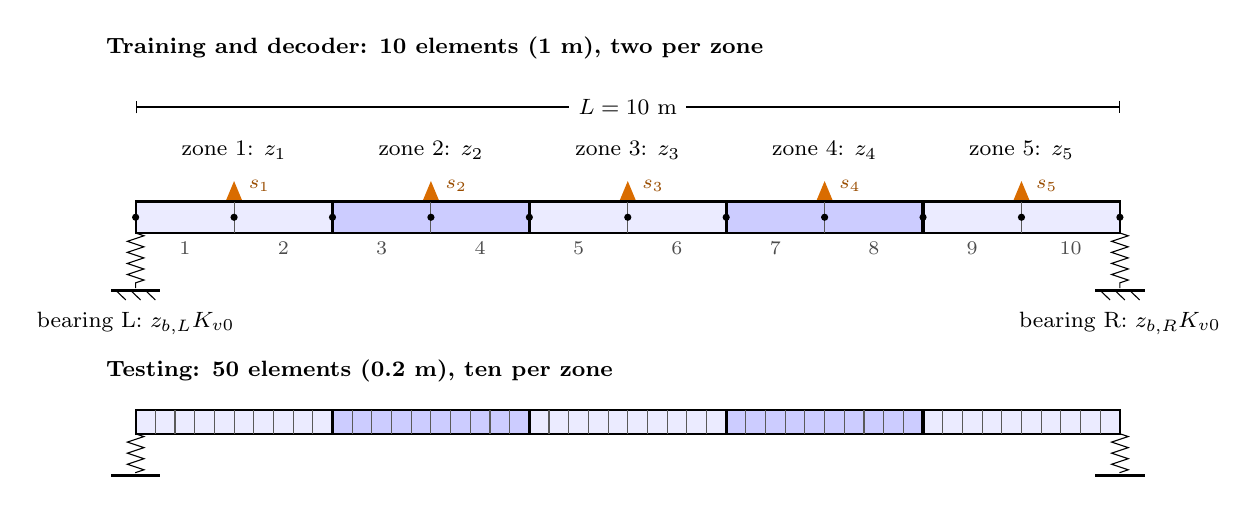
\begin{tikzpicture}[>=Stealth,font=\small,x=1.25cm,y=1cm]
  % ---- model used for training (decoder): 10 elements, 5 zones ----
  \node[anchor=west,font=\footnotesize\bfseries] at (-0.4,2.35) {Training and decoder: 10 elements (1~m), two per zone};
  \foreach \i/\c in {0/blue!8,1/blue!20,2/blue!8,3/blue!20,4/blue!8}{
    \fill[\c] (2*\i,0) rectangle (2*\i+2,0.4);
    \node[font=\footnotesize] at (2*\i+1,1.05) {zone \the\numexpr\i+1\relax: $z_{\the\numexpr\i+1\relax}$};
  }
  \draw[thick] (0,0) rectangle (10,0.4);
  \foreach \x in {1,3,5,7,9} \draw[gray!70!black] (\x,0) -- (\x,0.4);
  \foreach \x in {2,4,6,8} \draw[very thick] (\x,0) -- (\x,0.4);
  \foreach \x in {0,...,10} \fill (\x,0.2) circle (1.3pt);
  \foreach \e in {1,...,10} \node[font=\scriptsize,gray!60!black] at (\e-0.5,-0.2) {\e};
  \foreach \x/\k in {1/1,3/2,5/3,7/4,9/5}{
    \fill[orange!85!black] (\x-0.08,0.42) -- (\x+0.08,0.42) -- (\x,0.66) -- cycle;
    \node[font=\scriptsize,orange!60!black,anchor=west] at (\x+0.05,0.6) {$s_{\k}$};
  }
  \draw[|-|] (0,1.6) -- (10,1.6) node[midway,fill=white,font=\footnotesize] {$L=10$~m};
  \foreach \x/\lab in {0/{L},10/{R}}{
    \draw[decorate,decoration={zigzag,segment length=4,amplitude=3}] (\x,0) -- (\x,-0.7);
    \draw[thick] (\x-0.25,-0.73) -- (\x+0.25,-0.73);
    \foreach \h in {-0.2,-0.05,0.1} \draw (\x+\h,-0.73) -- (\x+\h+0.1,-0.85);
    \node[font=\footnotesize,anchor=north] at (\x,-0.88) {bearing \lab: $z_{b,\lab}K_{v0}$};
  }
  % ---- model used for testing: 50 elements ----
  \node[anchor=west,font=\footnotesize\bfseries] at (-0.4,-1.75) {Testing: 50 elements (0.2~m), ten per zone};
  \fill[blue!8] (0,-2.55) rectangle (2,-2.25); \fill[blue!20] (2,-2.55) rectangle (4,-2.25); \fill[blue!8] (4,-2.55) rectangle (6,-2.25);
  \fill[blue!20] (6,-2.55) rectangle (8,-2.25); \fill[blue!8] (8,-2.55) rectangle (10,-2.25);
  \draw[thick] (0,-2.55) rectangle (10,-2.25);
  \foreach \k in {1,...,49} \draw[gray!70!black] (\k*0.2,-2.55) -- (\k*0.2,-2.25);
  \foreach \x in {2,4,6,8} \draw[very thick] (\x,-2.55) -- (\x,-2.25);
  \foreach \x in {0,10}{
    \draw[decorate,decoration={zigzag,segment length=4,amplitude=3}] (\x,-2.55) -- (\x,-3.05);
    \draw[thick] (\x-0.25,-3.08) -- (\x+0.25,-3.08);
  }
\end{tikzpicture}
\caption{FE model of the revised case study (bridge S10 of Moliner et al., 2017, on elastic bearings). Top: model used for
training and embedded in the decoder, with 10 Euler--Bernoulli elements (numbered; dots mark the nodes), two per damage
zone. Bottom: finer model used to generate the test data, with 50 elements, ten per zone; the damage of a
damaged zone is concentrated in some of its elements (R1.5). The seven latent
variables are the stiffness factors of the five 2~m damage zones ($z_1,\dots,z_5$) and of the two bearings ($z_{b,L}$,
$z_{b,R}$), which scale the vertical springs $K_{v0}$. Five accelerometers ($s_1,\dots,s_5$) are placed at the centres of
the zones.}
\label{fig:bridge}
\end{figure}

\begin{table}[H]
\centering\small
\caption{Nominal values of the revised case study and their origin.}
\label{tab:specs}
\footnotesize
\begin{tabular}{p{3.0cm}p{6.6cm}p{5.0cm}}
\toprule
Item & Value & Origin \\
\midrule
Deck & reinforced concrete slab, span $L=10$~m, width $B=11.6$~m, depth $h=0.77$~m & bridge S10, Moliner et al.\ (2017), Table 2 \\
Elastic modulus & $E=3.4849\times10^{10}$~Pa & Moliner et al.\ (2017), Table 3 \\
Mass & 31\,301~kg/m (including ballast, sleepers and rails) & Moliner et al.\ (2017), Table 2 \\
Bending stiffness & $EI=1.54\times10^{10}$~N\,m$^2$, with $I=Bh^3/12$ & from the values above \\
Bearings & vertical springs, $\kappa=0.05$: $K_{v0}=9.5\times10^{6}$~kN/m each; free end rotations & $\kappa$: Moliner et al.\ (2017); range of
commercial bearings and free rotations: Erduran et al.\ (2022) \\
Discretization & 10 elements (training and decoder); 50 elements (test set B) & this work \\
\bottomrule
\end{tabular}
\end{table}

\begin{action}
New FE model of the bridge on elastic bearings \lines{xx--yy}, with Fig.~\tbd{x} (Fig.~\ref{fig:bridge}) and
Table~\tbd{x} (Table~\ref{tab:specs}).
\end{action}

% -----------------------------------------------------------------------------
\begin{rcomment}{3}
Methodology. Another limitation is the damage parametrization presented as a ``local'' loss of stiffness distributed within an element of a specific length. Considering the type of the bridge, this type of damage parametrization is not realistic, neither for steel bridges nor for RC. This point seems particularly important as the novelty of the proposed
methodology is presented as capturing the interconnectedness of damage scenarios. I recommend, in line with the comment above, including the support conditions in the formulation, which can enable to detect damage observed there.
\end{rcomment}

\begin{response}
We have revised the formulation in two ways.

\textit{Support conditions.} As recommended, the support conditions are now part of the formulation: the elastic bearings
are represented by vertical springs at both ends of the deck, each with its own stiffness reduction factor (R2.2,
Fig.~\ref{fig:bridge}), so that damage at the supports can be identified.

\textit{Damage parametrization.} The damage is no longer the stiffness loss of an individual element, but that of a damage
zone along the deck: the stiffness reduction factor of a zone scales the bending stiffness of all its elements (two in the
model used in training, ten in the testing model), independently of the discretization (Eq.~\eqref{eq:Kz}). This
equivalent stiffness reduction of a region of the deck is the usual representation of damage in vibration-based FE model
updating (Teughels et al., 2002; El-Borgi et al., 2005), and Moliner et al.\ (2017) reduce the elastic modulus of their
slab bridges by 10--20\% to account for cracking. To check this representation when the actual damage is concentrated,
the damage of every damaged zone in test set B is imposed on a group of contiguous elements of a 50-element model, from one
element (0.2~m) to the whole zone (2.0~m), with the same equivalent stiffness of the zone (R1.5, Eq.~\eqref{eq:localized}).
The model used in training cannot represent this localization.

The latent space now contains seven variables, corresponding to the stiffness factors of (i) the five zones along the
bridge deck and (ii) the two bearings (left and right). The new design of experiments (R1.6, Table~\ref{tab:doe}) focuses
on localized damage, i.e., damage at one, two or three of these seven locations, and it also includes healthy structures,
damage at four or five locations, and samples drawn uniformly over the whole parameter space. Every location and every
combination of locations, including combinations of deck and bearing damage, appears the same number of times. The
Gaussian copula captures the dependencies between these variables, e.g., between adjacent zones and between an end zone
and its bearing, which can partly compensate each other.
\tbd{VAE results for the bearings (benchmarks P4, P5 and P9).}
\end{response}

\begin{action}
New parametrization with zone and bearing stiffness factors \lines{xx--yy}; localized damage in the test data
\lines{xx--yy}.
\end{action}

% -----------------------------------------------------------------------------
\begin{rcomment}{4}
Methodology. The numerical case study, 5-elements simply supported beam is too simplistic. I would recommend at least
considering a more realistic case and testing the proposed method on a lab scale beam.
\end{rcomment}

\begin{response}
We agree that the original case study was too simplistic. We have revised it in two ways to bring it closer to a
realistic situation:
\begin{enumerate}[leftmargin=*,label=(\arabic*)]
\item A new FE model of a single-span bridge taken from the literature, discretized into 10 elements and supported on
elastic bearings, represented by vertical springs at both ends (R2.2).
\item The test data are generated with a much finer discretization (50 elements), as a real structure has many more DOFs
than the model embedded in the decoder, and every simulated structure has a perturbed mass (R1.2). The data are thus
generated with models that differ from the one used by the SciML method, as happens when a numerical model is used to
interpret the measurements of a real system.
\end{enumerate}
The validation on a laboratory-scale beam is not included in this revision. We now state it clearly as a limitation of the
present work, and we propose the validation with data from an experimental benchmark as future work.
\end{response}

\begin{action}
New case study \lines{xx--yy}; limitation and future work stated in the conclusions \lines{xx--yy}.
\end{action}

% =============================================================================
\section{Reviewer \#3}
% =============================================================================

\begin{rcomment}{}
In this manuscript, a novel probabilistic machine learning framework is presented for vibration-based damage
identification in civil infrastructure. The SHM approach employs a physics-informed Gaussian copula variational
autoencoder. The effectiveness of the framework is explored in detail and validated under various damage scenarios
using synthetic, noise-contaminated data of a simply supported bridge. The manuscript contains novel theoretical
developments that are worth publishing. Before publication, the following issues have to be addressed.
\end{rcomment}


% -----------------------------------------------------------------------------
\begin{rcomment}{1}
In Bayesian finite element model updating, the discrepancy between the physical structure and the parameterized
mathematical model (i.e., modeling error) dominates over sensor noise. The current validation assumes a perfectly known
baseline mass matrix and attributes all dynamic discrepancies to stiffness reductions (which are updated in the process)
and artificial Gaussian noise. To demonstrate the robustness of the PI-GCVAE, the authors must explore its sensitivity
to modeling errors (e.g., small random perturbations to the mass matrix) and investigate how such unmodeled dynamics
propagate into the posterior uncertainty bounds for the stiffness reduction factors.
\end{rcomment}

\begin{response}
We agree, and we followed the reviewer's suggestion. In the revised study, the baseline mass matrix is no longer
perfectly known. Every measurement, in the training, validation and test sets, comes from an as-built structure whose
mass differs from the nominal mass used by the decoder: the mass of each 1 m segment is multiplied by $1+\mu_s$, with
$\mu_s\sim\mathcal{N}(0,0.05^2)$ (Eq.~\eqref{eq:asbuilt}). In the second test set, the data also include a finer discretization and localized damage (R1.2).
The decoder keeps the nominal mass matrix, and the realizations of these perturbations are never available to the VAE.

\textit{Propagation into the posterior.} These unmodelled effects enter the inference through the likelihood
(Eqs.~\eqref{eq:discrepancy} and~\eqref{eq:nll}). We estimate their effect on the observations by simulation: the mass
perturbations alone change the frequencies with a standard deviation of 0.91--1.08\% and the mode shapes by up to
$3.5\times10^{-3}$ in $1-\mathrm{MAC}$ (Table~\ref{tab:budget}, Fig.~\ref{fig:budget}). Combined with the measurement
noise, the standard deviation of the log-frequency errors increases from 2.5\% to 2.66--2.72\%, and that of the
mode-shape components from 0.027--0.033 to 0.028--0.044. Since these values define the likelihood, the posterior bounds of the stiffness
factors widen consistently with what the decoder cannot represent, instead of attributing the mass deviations to
stiffness changes with false confidence. The calibration check on independent data confirms that the likelihood
describes the actual deviations (Fig.~\ref{fig:calib}). With this setup, the exact posteriors of the benchmark scenarios
have standard deviations of 0.03--0.13 for the deck zones and 0.03--0.05 for the bearings. Two of the test sets of R1.5
examine what happens when the modelling error is larger than assumed (twice the mass deviations) or
systematic (additional mass not included in the model).
\tbd{Posterior bounds and coverage of the VAE with modelling error; comparison with the exact posterior.}
\end{response}
\authornote{The reviewer states that modelling error dominates over sensor noise; with 5\% mass deviations, the
modelling error ($\approx$1\% on the frequencies; 1.2--1.8\% in test set B) is smaller than the identification noise (2.5\%); discuss this together with the larger
modelling errors of R1.5.}

\begin{action}
New subsection on modelling errors and their propagation \lines{xx--yy}; Table~\tbd{x} and Fig.~\tbd{x}.
\end{action}

% -----------------------------------------------------------------------------
\begin{rcomment}{2}
In the ``Sensitivity to $\gamma$ hyperparameter and model selection'' section, the hyperparameter $\gamma$, which
balances the data likelihood and the prior regularization, is calibrated based on the performance of the model on the
test dataset. This approach compromises the independence of the test set and results in overly optimistic performance
estimates. The optimal value of $\gamma$ must be selected using only the validation dataset. The authors need to
correct this methodological flaw and subsequently report the unbiased performance metrics on the completely unseen test
set.
\end{rcomment}

\begin{response}
We agree. In the revised formulation, $\gamma$ is no longer a tuned hyperparameter. In the submitted manuscript, the
frequency and mode-shape terms of the loss (Eqs.~(10)--(12)) were not scaled by the variance of their errors. In the
revised manuscript, every squared
discrepancy is divided by twice the variance of the corresponding error, $2\sigma^2$, which turns the data terms into the
negative log-likelihood of the measurements under Gaussian errors:
\begin{equation}
\mathcal{L}_{\text{ELBO}}(\bm\theta)\approx\mathcal{L}_{\text{freq}}(\bm\theta)+\mathcal{L}_{\text{MAC}}(\bm\theta)
+\gamma^2\mathcal{L}_{\text{PDF}}(\bm\theta),
\label{eq:loss}
\end{equation}
\begin{equation}
\begin{aligned}
\mathcal{L}_{\text{freq}}(\bm\theta)&=\frac{1}{N_{\text{train}}\cdot H}\sum_{i=1}^{N_{\text{train}}}\sum_{h=1}^{H}
\sum_{j=1}^{n_m}\frac{\big(\log f_{i,j}-\log\hat f_{i,j}^{h}\big)^2}{2\,\sigma_{f,j}^2},\\
\mathcal{L}_{\text{MAC}}(\bm\theta)&=\frac{1}{N_{\text{train}}\cdot H}\sum_{i,h,j}
\frac{1-\mathrm{MAC}_j\big(\bm\Phi_i,\hat{\bm\Phi}_i^{h}\big)}{2\,\sigma_{\Phi,j}^2},
\end{aligned}
\label{eq:nll}
\end{equation}
where $\sigma_{f,j}^2$ and $\sigma_{\Phi,j}^2$ are the variances of the errors of the $j$-th logarithmic frequency and of
each component of the $j$-th mode shape (normalized to unit norm). These variances include the measurement noise and the
modelling error, and they are estimated by simulation (R3.1); the revised manuscript also accounts for the weak
correlation between the errors of the different frequencies. As in the submitted manuscript, $\mathcal{L}_{\text{PDF}}$
is the logarithmic probability of the posterior samples under the estimated copula, i.e., minus the entropy of the
approximate posterior, which is now computed in closed form (R3.7). The scaling with $2\sigma^2$ has two consequences.
First, the relative weight of the frequency and mode-shape terms is set by the accuracy of each measured quantity.
Second, the data terms are measured in nats, on the same scale as
$\mathcal{L}_{\text{PDF}}$: with the uniform prior, Eq.~\eqref{eq:loss} with $\gamma=1$ is the negative ELBO (up to a
constant), whose minimizer is the Bayesian posterior within the variational family, whereas values $\gamma\neq1$
produce tempered posteriors without a probabilistic interpretation. We therefore fix $\gamma=1$ a priori. The trained model is selected on the validation set: we keep the weights with the
lowest negative ELBO, after a warm-up of 150 epochs in which the weight of the likelihood grows from 0.01 to 1. Every 20
epochs, the validation negative ELBO is estimated with 20 samples per observation and the same random numbers each time.
The learning rate, initially $5\times10^{-4}$, is halved after 200 epochs without an improvement larger than 0.002~nats,
and at $10^{-5}$ the same condition stops the training. 
% [ln z omitted in this revision, kept for later] The marginal family is compared with the same validation negative ELBO (R1.4). 
The test sets take no part in these criteria. The performance metrics on test set B are reported in
Table~\ref{tab:metricsB} (R1.3).

\textit{Role of $\gamma$ and sensitivity analysis.} For $\gamma\neq1$, the minimizer of Eq.~\eqref{eq:loss} is the
variational approximation of the tempered posterior $p_\gamma(\z|\m)\propto p(\m|\z)^{1/\gamma^2}\,p(\z)$: $\gamma<1$ sharpens the posterior (overconfident intervals) and $\gamma>1$ widens it (conservative intervals).
In the revised formulation, the width of the posterior is therefore set by the statistics of the measurement and
modelling errors in the likelihood (R1.2, R1.3), not by $\gamma$. To show this, and to document how sensitive the
results are to this choice, we add a sensitivity analysis in which the model is retrained with
$\gamma\in\{0.5,0.75,1,1.5,2\}$ ($\gamma^2$ from 0.25 to 4), all other settings unchanged. For each value we report,
on the validation set only, the empirical coverage and the MACE of the credible intervals, the error of the posterior
mean, and the agreement with the exact posteriors computed with the same $\gamma$. We expect the posterior means to be
almost insensitive to $\gamma$ and the coverage to be closest to its nominal value at $\gamma=1$. This analysis
illustrates the effect of $\gamma$ and is not used to select it: $\gamma=1$ is kept for all the reported results.
\tbd{Results of the sensitivity analysis: coverage and MACE vs.\ $\gamma$ (figure), error of the posterior mean.}
\end{response}
\authornote{(i) Sensitivity study not run yet: 4 additional trainings ($\gamma=0.5$, 0.75, 1.5, 2). (ii) The submitted
manuscript reports $\gamma=0.30$ (confirmed with manuscript\_old.tex and the archived run Beta0.3), and its selection
relied on MSE, MAE and coverage values affected by the array-shape error described in R1.3. (iii) Test set B is misspecified (localized damage, R1.5), and $\gamma$ slightly above 1 may calibrate better
there (power/generalized posteriors, e.g., Gr\"unwald and van Ommen, 2017). If we want to discuss this, we need a
validation set generated like test set B, so that the test sets are still not used for any choice. }
% (iv) During
% development we inspected test-set results of several marginal families, and the idea of working in $\ln z$ came from best
% fits to the exact marginals of test set A. The criterion written here is validation-only, but we cannot claim that the
% test sets were seen only once or call the metrics fully unbiased; decide how to state this.
%}

\begin{action}
Section ``Sensitivity to $\gamma$ hyperparameter and model selection'' rewritten \lines{xx--yy}.
\end{action}

% -----------------------------------------------------------------------------
\begin{rcomment}{3}
Within the Bayesian setting, the posterior is heavily dependent on the choice of the prior $p(\z)$. The formulation
assumes a bounded uniform prior $\mathcal{U}[0.5,1.0]$. At the same time, the synthetic training dataset is generated
by uniformly sampling the same space. In actual SHM applications, severe damage is highly improbable; thus, a realistic
prior should strongly penalize large reductions in stiffness. The authors should clarify the distinction between the
generative sampling density used for training (which might be uniform to prevent class imbalance) and the theoretical
Bayesian prior incorporated in the ELBO loss. Can the current framework accommodate an informative, non-uniform prior
while training on uniform data? A brief discussion on this decoupling is necessary.
\end{rcomment}

\begin{response}
We now discuss this point explicitly. Two different distributions play a
role:
\begin{itemize}[leftmargin=*]
\item The \emph{prior} $p(\z)$ is part of the Bayesian model. It enters the loss through the negative ELBO of each
observation,
\begin{equation}
-\mathrm{ELBO}(\m)=\mathbb{E}_q\big[\mathrm{NLL}(\z;\m)\big]+\mathbb{E}_q\big[\log q(\z|\m)\big]
-\mathbb{E}_q\big[\log p(\z)\big],
\label{eq:elbo_prior}
\end{equation}
and through the reference posterior.
\item The \emph{sampling density} of the training data (the DoE) only determines which observations the encoder sees
during training. The loss is an average over observations of Eq.~\eqref{eq:elbo_prior}, and for each observation its
minimizer is the posterior $p(\z|\m)\propto p(\m|\z)\,p(\z)$, independently of how often that observation appears in the
training set. The DoE therefore determines where the amortized encoder is accurate, not which posterior it targets.
\end{itemize}
The revised study makes this decoupling explicit: the prior is uniform on $[0.45,1]^7$, whereas the DoE is a balanced
mixture of healthy and localized damage scenarios (R1.6) that is far from uniform (two thirds of the parameters lie in
$[0.95,1]$). For a uniform prior, the last term of Eq.~\eqref{eq:elbo_prior} is constant, which is why the loss only
contains the likelihood and the entropy. An informative prior, e.g., one that penalizes large stiffness reductions,
only requires adding $-\mathbb{E}_q[\log p(\z)]$ to the loss, estimated with the same samples of $q$, and using the same
prior in the reference posterior. Neither the training data nor the architecture change.
\end{response}
\authornote{optional: demonstrate an informative prior on one benchmark.}

\begin{action}
New paragraph on the prior and the sampling density of the training data \lines{xx--yy}, with
Eq.~\eqref{eq:elbo_prior}.
\end{action}

% -----------------------------------------------------------------------------
\begin{rcomment}{4}
The identification relies on the first 5 modes to estimate damage in a 5-element beam. The accuracy of Bayesian
parameter estimation is fundamentally dictated by the information content of the measured data. While higher modes
offer better spatial resolution for localized damage, they are increasingly contaminated by measurement noise. A brief
sensitivity analysis or discussion of how the number of modes used affects parameter identifiability and the width of
the posterior uncertainty bounds is needed. How does the proposed VAE handle the transition to a severely ill-posed
scenario when fewer modes are available?
\end{rcomment}

\begin{response}
We agree, and we carried out a sensitivity analysis of the measurement setup with the data generator of the revised
study.

\textit{Distinguishability of the modes.} The modes must be distinguishable at the sensors, otherwise they cannot be
paired with those of the model. Over random damage states, the largest MAC between two different modes at the sensors is
0.24 for the six sensors at the zone boundaries of the submitted version and 0.07 for five sensors at the
zone centres, which we adopt.

\textit{Exact posteriors.} For five setups, we computed the exact posteriors of five benchmark scenarios, each setup with
its own calibrated likelihood (Table~\ref{tab:modes}). With fewer modes, the posteriors widen (mean standard deviation
0.046--0.075 with five modes and 0.062--0.088 with three), and the probability assigned to the true damage location
decreases. For the severe damage of zone 1 in P1 ($z_1=0.56$), the posterior probability that zone 1 is damaged ($z_1<0.85$) is 1.00 with five modes,
0.87 with three modes and 0.77 with three modes and three sensors, while that of its mirror zone grows from 0.08 to 0.34 and 0.50. In P9, the mirror
probability is 0.39, 0.26 and 0.49, so it does not vary monotonically in a single noise realization. The transition to ill-posedness therefore appears as wider and skewed marginals and more ambiguity between
symmetric locations. The bearing of P4 remains identified in all setups (standard deviation 0.022--0.052), because the bearings affect every mode.

\textit{Adopted setup.} We adopted five vertical accelerometers at the zone centres and the first five modes (up to
155~Hz for the healthy bridge), in which the modes are well separated at the sensors and the mesh error of the decoder is small
(Table~\ref{tab:mesh}). With this setup, the posteriors keep a substantial uncertainty (standard deviations up to 0.13 for the deck zones), so the
identification is genuinely probabilistic.

\textit{The VAE with less information.} To show how the VAE handles fewer data, we also train it with three modes and,
with five modes, with the frequencies only. 
% Before training, we checked the marginal family against the exact posteriors
% of 131 test scenarios (best fit of each marginal, without the encoder). The mean Wasserstein-1 distance of one Gaussian in
% $\ln z$ to the exact marginals is 0.0013 with five modes, 0.0023 with three modes and 0.0021 with the frequencies only;
% for one Gaussian in $z$, it is 0.0033, 0.0053 and 0.0048.
\tbd{Comparison between the VAE and the exact posteriors with five modes, three modes and frequencies only.}
\end{response}

\begin{table}[H]
\centering\small
\caption{Exact posteriors of benchmarks P1, P3, P4, P6 and P9 for five measurement setups (one noise realization per
setup; calibrated likelihood of each setup): range of the mean posterior standard deviation and of the widest 95\%
credible interval over the benchmarks, and posterior probability that the true damaged parameter and its mirror have
$z<0.85$ (P1: zone 1, true $z_1=0.56$, mirror zone 5; P4: left bearing, true $z_{b,L}=0.55$, mirror right bearing; P9:
zone 2, true $z_2=0.58$, mirror zone 4).}
\label{tab:modes}
\footnotesize\setlength{\tabcolsep}{4pt}
\begin{tabular}{lccccc}
\toprule
 & & Widest 95\% & \multicolumn{3}{c}{Probability of $z<0.85$: true / mirror} \\
\cmidrule(l){4-6}
Setup & Mean std & interval & P1 & P4 & P9 \\
\midrule
7 sensors (with supports), 5 modes & 0.042--0.065 & 0.24--0.37 & 0.999 / 0.235 & 1.000 / 0.006 & 1.000 / 0.215 \\
5 sensors, 5 modes (adopted) & 0.046--0.075 & 0.25--0.49 & 1.000 / 0.081 & 1.000 / 0.053 & 0.999 / 0.394 \\
5 sensors, 4 modes & 0.051--0.066 & 0.24--0.45 & 1.000 / 0.165 & 1.000 / 0.028 & 0.999 / 0.056 \\
5 sensors, 3 modes & 0.062--0.088 & 0.34--0.50 & 0.868 / 0.337 & 1.000 / 0.167 & 0.962 / 0.261 \\
3 sensors, 3 modes & 0.068--0.104 & 0.36--0.52 & 0.767 / 0.501 & 1.000 / 0.112 & 0.830 / 0.490 \\
\bottomrule
\end{tabular}
\end{table}
\authornote{one noise realization per setup; replicas would smooth non-monotone values such as the mirror probability of
P9. The values come from the script identifiability\_setups.py.}

\begin{action}
New paragraph and table on the influence of the number of modes and sensors \lines{xx--yy}.
\end{action}

% -----------------------------------------------------------------------------
\begin{rcomment}{5}
The readability of the manuscript would benefit from a dedicated flowchart illustrating the synthetic dataset
generation process (parameter sampling, forward eigenvalue solution, noise injection), distinguishing clearly between
the offline training phase and the online inference phase.
\end{rcomment}

\begin{response}
We agree, and we added the flowchart of Fig.~\ref{fig:flowchart}, which distinguishes three stages:
\begin{itemize}[leftmargin=*]
\item \emph{Offline, synthetic data generation.} The damage states are sampled with the design of experiments (R1.6);
each one is combined with a new as-built structure (random mass distribution, R1.2), its natural frequencies and mode
shapes are computed by solving the FE eigenvalue problem (with the FE model of the decoder for the training and
validation data, and with a refined FE model with localized damage for the test data, R1.5), and measurement noise is
added at the sensors.
\item \emph{Offline, physics-informed training.} The encoder maps the modal data to the Gaussian copula posterior; its
samples are passed through the embedded eigenvalue solver, and the negative ELBO (calibrated likelihood and entropy) is
minimized. The true damage states are never used in the loss.
\item \emph{Online, damage identification.} The trained encoder maps the measured modal data of the structure to the
posterior of the stiffness factors in a single forward pass, without solving the FE model, which gives the damage
assessment (posterior mean, credible intervals and healthy or damaged classification, R1.6).
\end{itemize}
\end{response}

\begin{figure}[H]
\centering
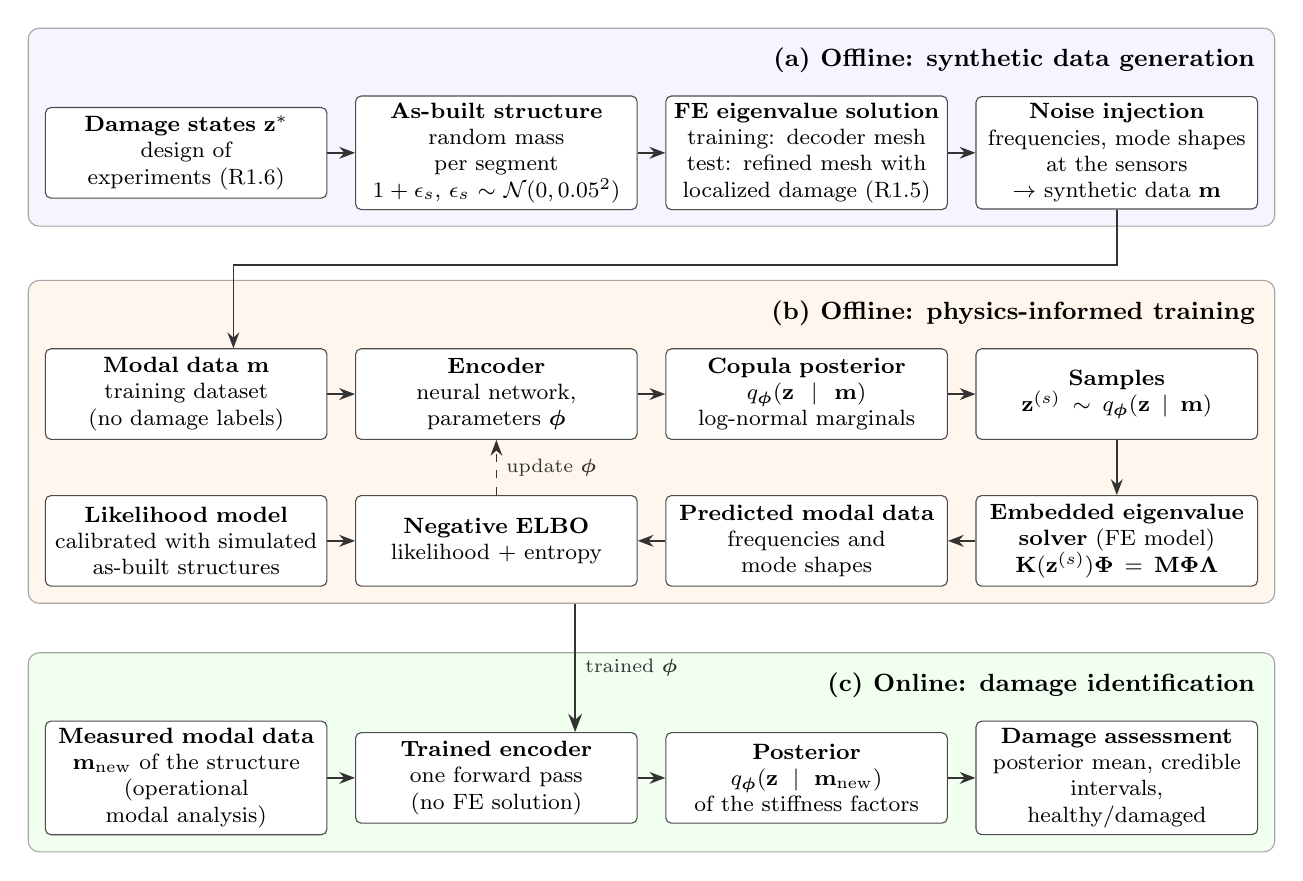
\begin{tikzpicture}[>=Stealth,font=\footnotesize,node distance=4mm and 3.5mm,
  box/.style={draw=black!70,rounded corners=2pt,align=center,fill=white,inner sep=2.5pt,minimum height=1.15cm,text width=3.4cm,execute at begin node={\hyphenpenalty=10000\relax\exhyphenpenalty=10000\relax}},
  arr/.style={->,semithick,black!80},
  ttl/.style={font=\bfseries\small,anchor=south east,inner sep=1pt},
  panel/.style={draw=black!35,rounded corners=4pt,inner sep=6pt}]
% ------------------------------------------------------------------ (a) data generation
\node[box] (doe) {\textbf{Damage states} $\z^*$\\design of experiments (R1.6)};
\node[box,right=of doe] (ab) {\textbf{As-built structure}\\random mass per segment\\$1+\epsilon_s$, $\epsilon_s\sim\mathcal{N}(0,0.05^2)$};
\node[box,right=of ab] (fe) {\textbf{FE eigenvalue solution}\\training: decoder mesh\\test: refined mesh with\\localized damage (R1.5)};
\node[box,right=of fe] (noise) {\textbf{Noise injection}\\frequencies, mode shapes\\at the sensors\\$\to$ synthetic data $\m$};
\node[ttl] (ta) at ([yshift=2.5mm]noise.north east) {(a) Offline: synthetic data generation};
\draw[arr] (doe)--(ab); \draw[arr] (ab)--(fe); \draw[arr] (fe)--(noise);
% ------------------------------------------------------------------ (b) training
\node[box,below=19mm of doe] (m) {\textbf{Modal data} $\m$\\training dataset\\(no damage labels)};
\node[box,right=of m] (enc) {\textbf{Encoder}\\neural network,\\parameters $\bm\phi$};
\node[box,right=of enc] (q) {\textbf{Copula posterior}\\$q_{\bm\phi}(\z\mid\m)$\\log-normal marginals};
\node[box,right=of q] (samp) {\textbf{Samples}\\$\z^{(s)}\sim q_{\bm\phi}(\z\mid\m)$};
\node[box,below=7mm of samp] (eig) {\textbf{Embedded eigenvalue}\\\textbf{solver} (FE model)\\$\mathbf{K}(\z^{(s)})\bm\Phi=\mathbf{M}\bm\Phi\bm\Lambda$};
\node[box,left=of eig] (pred) {\textbf{Predicted modal data}\\frequencies and\\mode shapes};
\node[box,left=of pred] (loss) {\textbf{Negative ELBO}\\likelihood + entropy};
\node[box,left=of loss] (cal) {\textbf{Likelihood model}\\calibrated with simulated\\as-built structures};
\node[ttl] (tb) at ([yshift=2.5mm]samp.north east) {(b) Offline: physics-informed training};
\draw[arr] (m)--(enc); \draw[arr] (enc)--(q); \draw[arr] (q)--(samp); \draw[arr] (samp)--(eig);
\draw[arr] (eig)--(pred); \draw[arr] (pred)--(loss); \draw[arr] (cal)--(loss);
\draw[arr,dashed] (loss.north) -- node[right,font=\scriptsize]{update $\bm\phi$} (enc.south);
\draw[arr] (noise.south) -- ++(0,-7mm) -| ([xshift=6mm]m.north);
% ------------------------------------------------------------------ (c) online
\node[box,below=17mm of cal] (meas) {\textbf{Measured modal data}\\$\m_{\mathrm{new}}$ of the structure\\(operational modal analysis)};
\node[box,right=of meas] (tenc) {\textbf{Trained encoder}\\one forward pass\\(no FE solution)};
\node[box,right=of tenc] (post) {\textbf{Posterior}\\$q_{\bm\phi}(\z\mid\m_{\mathrm{new}})$\\of the stiffness factors};
\node[box,right=of post] (out) {\textbf{Damage assessment}\\posterior mean, credible\\intervals, healthy/damaged};
\node[ttl] (tc) at ([yshift=2.5mm]out.north east) {(c) Online: damage identification};
\draw[arr] (meas)--(tenc); \draw[arr] (tenc)--(post); \draw[arr] (post)--(out);
% ------------------------------------------------------------------ panels
\begin{scope}[on background layer]
\node[panel,fill=blue!4,fit=(ta)(doe)(noise)] (pa) {};
\node[panel,fill=orange!7,fit=(tb)(m)(samp)(eig)(cal)] (pb) {};
\node[panel,fill=green!6,fit=(tc)(meas)(out)] (pc) {};
\end{scope}
\draw[arr,thick] ([xshift=10mm]tenc.north |- pb.south) -- node[right,font=\scriptsize]{trained $\bm\phi$} ([xshift=10mm]tenc.north);
\end{tikzpicture}
\caption{Methodology: (a) generation of the synthetic data, (b) offline training of the encoder through the embedded
eigenvalue solver, without the true damage states, and (c) online identification of a new structure with the trained
encoder.}
\label{fig:flowchart}
\end{figure}

\begin{action}
New flowchart (Fig.~\tbd{x}, Fig.~\ref{fig:flowchart}) \lines{xx--yy}.
\end{action}

% -----------------------------------------------------------------------------
\begin{rcomment}{6}
Equation 11 ($\mathcal{L}_{\mathrm{freq}}$): The notation $\mathbf{K}_{\mathrm{G}}$ in the decoder function is slightly
confusing since Eq. 5 defines $\hat{\mathbf{K}}_{\mathrm{G}}(\z)$ as the updated stiffness matrix. Please clarify if
$\mathbf{K}_{\mathrm{G}}$ refers to the baseline assembled matrix to avoid confusion with the damaged global matrix.
\end{rcomment}
\pending

% -----------------------------------------------------------------------------
\begin{rcomment}{7}
Sample size in training ($H=1$): In the ``Architecture design and training specifications'' section, it is stated that
a single sample ($H=1$) is drawn during training. While common in VAEs with large batch sizes, please briefly justify why
$H=1$ is sufficient to approximate the expectations in the ELBO loss.
\end{rcomment}

\begin{response}
In the revised implementation, we draw $H=6$ samples of the approximate posterior per observation. With batches of 256
observations, each gradient step uses 1\,536 samples. The Monte Carlo estimate of the loss is unbiased for any $H$, and
$H$ only affects the variance of the gradients. This variance is further reduced because the entropy is computed
exactly, in closed form (Eq.~\eqref{eq:loss}), so that the samples are only used for the expectation of the negative
log-likelihood. The samples are obtained with the closed-form quantile of the truncated normal distribution at the uniform
variables produced by the Gaussian copula. This expression is differentiable with respect to the encoder outputs, and it
replaces the rejection sampling of the submitted version.
% $H$ only affects the variance of the gradients. This variance is further reduced because the entropy is computed
% exactly, in closed form (Eqs.~\eqref{eq:marginal} and~\eqref{eq:loss}), so that the samples are only used for the
% expectation of the negative log-likelihood. The samples are obtained with the closed-form quantile of
% Eq.~\eqref{eq:marginal} at the uniform variables produced by the Gaussian copula. This expression is differentiable with
% respect to the encoder outputs, and it replaces the rejection sampling of the submitted version.
\end{response}
\authornote{optional: a short check of the sensitivity of the results to $H$.}

\begin{action}
Training specifications updated \lines{xx--yy}.
\end{action}

% -----------------------------------------------------------------------------
\begin{rcomment}{8}
Hardware and computational cost: Please report the hardware specifications and the approximate wall-clock time
required for the 11,000 training epochs to provide a practical sense of the computational cost of differentiating the
eigenvalue solver.
\end{rcomment}
\pending
\authornote{report the hardware and wall-clock time of the final training on the GPU server (NVIDIA Quadro GV100 and L40S GPUs; the eigenproblems are solved on the CPU in double precision), measured on an otherwise idle GPU.}

% =============================================================================
\section{References cited in this letter}
% =============================================================================
{\small
\begin{itemize}[leftmargin=*,label={}]
\item El-Borgi, S., Choura, S., Ventura, C., Baccouch, M., Cherif, F. (2005). Modal identification and model updating of a reinforced concrete bridge. Smart Struct.\ Syst.\ 1(1), 83--101.
\item Erduran, E., Nordli, C., Gonen, S. (2022). Effect of elastomeric bearing stiffness on the dynamic response of railway bridges considering vehicle--bridge interaction. Appl.\ Sci.\ 12(23), 11952.
\item Luo, L., Sun, L., Song, M., Liu, J., Li, Y., Xia, Y. (2025). Joint load-parameter-response identification using a physics-encoded neural network. Mech.\ Syst.\ Signal Process.\ 230, 112597.
\item Moliner, E., Mart\'{\i}nez-Rodrigo, M.D., Museros, P. (2017). Dynamic performance of existing double track railway bridges at resonance with the increase of the operational line speed. Eng.\ Struct.\ 132, 98--109.
\item Teughels, A., Maeck, J., De Roeck, G. (2002). Damage assessment by FE model updating using damage functions. Comput.\ Struct.\ 80(25), 1869--1879. \tbd{check the volume and pages}
\item \tbd{Refs.~39 and 41 are those of the manuscript (Fernandez-Navamuel et al., 2025; Fernandez-Navamuel et al., 2026).}
\end{itemize}
\vspace{-\baselineskip}
\renewcommand{\bibsection}{}
\setlength{\bibsep}{0.3ex}
\bibliographystyle{plainnat}
\bibliography{references_letter}
}

\end{document}
